\documentclass[12pt]{article}

\usepackage[left=1in, right=1in, top=1in, bottom=1in, headheight=1in]{geometry}

\usepackage[document]{ragged2e}
\usepackage{setspace}

%% font of the document is to be sans serif.
\usepackage{fontspec}
\setmainfont{Atkinson Hyperlegible}
\setmonofont[Scale=0.85]{JetBrainsMono Nerd Font}

\usepackage{titling}
\usepackage{amsmath}
\usepackage{listings}
\usepackage{algpseudocode}
\usepackage{graphicx}
\usepackage{subcaption}
\usepackage[countmax]{subfloat}
\usepackage{float}
\usepackage[framemethod=tikz]{mdframed}
\usepackage{pdfpages}
\usepackage{shellesc}
% \usepackage{microtype}

\usepackage{xcolor}
% Nord color theme - https://www.nordtheme.com/
% See https://www.nordtheme.com/docs/colors-and-palettes for colors and style guides.
% Polar Night
\definecolor{nord0}{RGB}{46, 52, 64}
\definecolor{nord1}{RGB}{59, 66, 82}
\definecolor{nord2}{RGB}{67, 76, 94}
\definecolor{nord3}{RGB}{76, 86, 106}
% Snow Storm
\definecolor{nord4}{RGB}{216, 222, 233}
\definecolor{nord5}{RGB}{229, 233, 240}
\definecolor{nord6}{RGB}{236, 239, 244}
% Frost
\definecolor{nord7}{RGB}{143, 188, 187}
\definecolor{nord8}{RGB}{136, 192, 208}
\definecolor{nord9}{RGB}{129, 161, 193}
\definecolor{nord10}{RGB}{94, 129, 172}
\definecolor{nord11}{RGB}{191, 97, 106}
% Aurora
\definecolor{nord12}{RGB}{208, 135, 112}
\definecolor{nord13}{RGB}{235, 203, 139}
\definecolor{nord14}{RGB}{163, 190, 140}
\definecolor{nord15}{RGB}{180, 142, 173}

\usepackage{moreverb}

\sloppy

%TC:ignore
\immediate\write18{echo -n $(texcount -total -sum -brief \jobname.tex) > count.tex}
%TC:endignore

\lstset{
	basicstyle = \footnotesize\ttfamily,
	columns = fullflexible,
	showlines=true,
	backgroundcolor=\color{nord6},   % choose the background color; you must add \usepackage{color} or \usepackage{xcolor}
	captionpos=b,                    % sets the caption-position to bottom
	commentstyle=\color{nord3}\textit,    % comment style
	% deletekeywords={...},            % if you want to delete keywords from the given language
	escapeinside={\%*}{*},          % if you want to add LaTeX within your code
	extendedchars=true,              % lets you use non-ASCII characters; for 8-bits encodings only, does not work with UTF-8
	keepspaces=true,                 % keeps spaces in text, useful for keeping indentation of code (possibly needs columns=flexible)
	keywordstyle=\color{nord9}\bfseries,       % keyword style
	otherkeywords={*} % if you want to add more keywords to the set
	numbers=left,                    % where to put the line-numbers; possible values are (none, left, right)
	numbersep=5pt,                   % how far the line-numbers are from the code
	numberstyle=\tiny\color{nord15}, % the style that is used for the line-numbers
	showspaces=false,                % show spaces everywhere adding particular underscores; it overrides 'showstringspaces'
	showstringspaces=false,          % underline spaces within strings only
	showtabs=false,                  % show tabs within strings adding particular underscores
	stepnumber=1,                    % the step between two line-numbers. If it's 1, each line will be numbered
	stringstyle=\color{nord14}, % string literal style
	tabsize=2,	                   % sets default tabsize to 2 spaces
	title=\lstname,                  % show the filename of files included with \lstinputlisting; also try caption instead of title
	columns=fixed                    % Using fixed column width (for e.g. nice alignment)
}
\surroundwithmdframed[
	hidealllines=true,
	backgroundcolor=nord6,
	innerleftmargin=8pt,
	skipbelow=0,
	innertopmargin=0.75em,
	innerbottommargin=-1.5em]{lstlisting}

\usepackage{fancyhdr}

\usepackage{csquotes}
\usepackage[hidelinks, urlcolor=blue]{hyperref}
\usepackage{url}
\usepackage[shortlabels]{enumitem}

\usepackage[section, numbib, nottoc]{tocbibind}
\usepackage[natbib, style=ieee, url=true, doi=true]{biblatex}
\usepackage[title, titletoc]{appendix}
\usepackage{tocloft}


\tolerance=1
\emergencystretch=\maxdimen
\hyphenpenalty=10000
\hbadness=10000

% \setcounter{tocdepth}{2}

% Apply larger line spacing
\linespread{1}

% no indentation on new line, use linebreaks instead
\setlength{\parindent}{0pt} 
\setlength{\parskip}{0.5em}

%  Remove additional itemize indent
\setlist[itemize]{leftmargin=1em}

% Add references / bibliography
\addbibresource{references.bib}

\title{{\huge TSR}\vspace{0.5em}\\
Designing an off-road, user-centred routing algorithm to promote on-foot transport.}
\author{George Pestell (200007413)}
\date{} 

\begin{document}

\fancyhead[L]{Student ID: 200007413}
\fancyhead[C]{TSR}
\fancyhead[R]{\thepage}
\fancyfoot{}

\makeatletter
\begin{titlepage}
  \centering

  \vspace*{\fill}

  \textbf{\large{\thetitle}}

  
\includegraphics[width=0.5\textwidth]{./assets/01-standard-vertical-black-text.png}

  \textbf{\large{\theauthor}}

  \vspace{0.2cm}

  \large{Supervisor: Prof. Graham Kirby}
  \vspace{0.8cm}

  \large{Department of Computer Science\\
    University of St. Andrews}

  \large{Date Submitted: \today}

  \vspace{0.8cm}

  \large{This dissertation is submitted for the degree of \\
    Integrated Masters in Computer Science}


  \vspace*{\fill}

\end{titlepage}
\makeatother

\pagebreak
\pagenumbering{roman}

\section*{Abstract}

In this dissertation, the challenge of improving the accessibility of off-road walking and running by developing a route-planner unrestricted to solely utilizing roads/paths. Building on modern studies in robotics and search-and-rescue, in addition to ideas developed in a seminal thesis project at the University of St. Andrews on the same topic, a modular cost-function framework is introduced. This framework integrates diverse map-related data, allowing mathematical models of factors impacting route selection preferences such as the factors impacting walking speed. Example cost-function presets are evaluated, demonstrating the flexibility of such an approach. Finally, the potential for further research and exploration are discussed in detail.

\section*{Declaration}

I declare that the material submitted for assessment is
my own work except where credit is explicitly given to
others by citation or acknowledgement. This work was
performed during the current academic year except where
otherwise stated.

The main text of this project report is
10074words long, including project specification and plan.

In submitting this project report to the University of St
Andrews, I give permission for it to be made available for
use in accordance with the regulations of the University
Library. I also give permission for: the title and abstract to
be published; and for copies of the report to be made and
supplied at cost to any bona fide library or research
worker; and to be made available on the World Wide Web.
I retain the copyright in this work.

\pagebreak
\tableofcontents

\pagebreak
\pagestyle{fancy}

\section{Introduction}
\pagenumbering{arabic}

Route planner applications enable users to select two points on the Earth's surface, and produces output representing a suggested set of points between the two points the router has deemed optimal. They are ubiquitous in both business and consumer settings --- with Google Maps alone seeing over one billion users annually \autocite{google2019keyword}.

However, existing tools are consistently restricted to searching for routes over pre-defined paths and roads. Whilst ideal for motor vehicles, on-foot travel offers far greater flexibility in traversable terrain that is underutilized by these tools. This limitation contributes to the low uptake of walking, which is a far healthier and environmentally friendly form of transportation \autocite{ukgov2021travel}. Studies show that the perception of a lack of available walking routes, and perceived danger of sharing roads with cars is a primary deterrent \autocite{ek2021motives,singleton2019walking}.

Previous research into off-road route planning has been mostly restricted to specialist fields like robotics and search-and-rescue applications \autocite{perkins2013fielddstar,zhao2024searchrescue}. \textcite{evans2023tsr} made a notable attempt to generalize off-road route planning for pedestrians, creating a custom cost-function, allowing features impacting walking speed to be modelled. This project aims to develop and document a broader cost framework, enabling complex modelling of relationships between data and any factor influencing route selection or safety. By generating safe, individualized routes, this project seeks to make on-foot travel more accessible and appealing for everyday transport.

\section{Context Survey}

\subsection{GIS Software}

GIS software integrates diverse mapping-related data sources. Tools such as ArcGIS offer visualization and analysis, with plugins enabling data relationships to be modelled. These large scale applications use databases to store map data tiles in layers, enabling efficient storage and retrieval relevant to a particular area. GDAL \autocite{gdal} enhances the flexibility of GIS by storing data in files. GDAL offers a suite of command line tools, and a C++ library, for working with individual data files. Tiling is supported. GDAL files require specialist file formats such as GeoTiff and GeoJSON, storing useful location and resolution metadata.

\subsubsection{GIS API Standards}

The catalogue service for the web (WCS) is an API specification created by the Open Geospatial Consortium \autocite{ogc_wcs}, enabling consistent interaction with GIS software using HTTP requests.

Clients interact with WCS services through fetching a metadata end-point \texttt{GetCapabilities} --- returning an XML document containing the features enabled by the service. A standard WCS HTTP request follows the basic format \texttt{https://BASEURL?SERVICE=WCS\&VERSION=2.0.2\&REQUEST=GetCapabilities}.

A web map service (WMS) is comparable to a WCS, also developed by the Open Geospatial Consortium. These API services solely offer GIS raster images. Endpoints include \texttt{GetCapabilities} and \texttt{GetMap} \autocite{ogc_wms}.

\subsection{Computer Vision}

Computer vision is a field of artificial intelligence, enabling computers to analyse images. Through image processing and pattern recognition, meaningful information can be extracted. One common use for computer vision technologies is edge detection, which can be outputted as vector representations of the boundaries between data values. For off-road routing, this is of particular interest in accurately determining the boundaries of raster features to improve the resolution of routes generated.

\subsection{Shortest Path Search Algorithms}

Shortest-path algorithms aim to find the route with the lowest cost between two nodes in a graph. Costs are defined by weights applied to edges, nodes, or other graph elements, representing quantifiable metrics such as distance, or travel difficulty. These algorithms are crucial for route planning, providing the foundational algorithms for calculating optimal routes, and for taking into consideration complex user-defined preferences in their weights. The following will outline some key algorithms.

\subsubsection{Dijkstra's Algorithm}

Dijkstra's famous algorithm \autocite{dijkstra1959} is guaranteed to find the optimal route, by calculating the minimum non-negative costs from a source node to all other nodes. Iteratively evaluating connected nodes, the minimum costs are updated as each path is searched, and shorter paths are found.

Uniform cost search describes an optimized implementation of Dijkstra's algorithm, using a priority queue of searched costs to only store the true minimum cost once it is found. This optimized implementation has been found to have a time complexity of $\mathcal{O} ((E + N) \log{N})$, where $E$ represents edges and $N$ nodes.

Costs must be non-negative, as Dijkstra's and Uniform Cost Search both follow a best-first strategy by following the current minimum cost node from the search node. Allowing negative costs may enable a node that has a high cost to reach not to be searched fully, despite the path to the target node being negative, and thus the shortest path.

% Linking in with the project and why it's useful for a route planner
\subsubsection{A* Algorithm}

A* enhances Dijkstra's algorithm with heuristics to guide searches toward the target, minimizing unnecessary calculations. Heuristics predict remaining costs to the target and must be admissible (not overestimating true costs) to ensure accuracy. While terrain-sensitive routing could benefit from this approach, developing admissible heuristics for complex cost functions remains challenging.

\subsection{Search Graph Representations}

Route planners rely on graph structures to represent the environment. For road networks, topological graphs simplify representation by focusing on connections, reducing nodes and data storage requirements. For off-road scenarios, geometric graphs better preserve real-world angles and distances, offering greater accuracy in areas where users can freely traverse terrain.

\subsection{Surface Meshes}

Surface meshes represent 3D objects using vertices, edges, and faces, with triangular irregular networks (TINs) being the industry standard for terrain modelling. DEMs, created through technologies like LIDAR or radar, offer foundational elevation data. Raster DEMs provide grids of elevation points, while vector contour lines require conversion for mesh generation. TINs constructed from DEMs balance geometric accuracy with computational efficiency.

\subsection{Digital Elevation Models}

Digital elevation models (DEMs) are the datasets constructed by scanning technologies to represent the topography of the earth's surface.

Large-scale terrain meshes of the earth's surface are usually constructed using radar data, that is restricted to 2.5D measurements, as it is restricted to a single point of measurement. LIDAR data is more commonly used for smaller, 3D terrain models, as multiple angles enable multiple elevation points to capture 3D geometry, at the cost of a larger volume of data needing to be stored and processed. Additionally, LIDAR suffers from limited coverage and licence restrictions, due to the specialist technologies required to create it.

The most common DEM format is raster data, providing a grid of elevation points created from the raw scanning data. Contour lines offer a vector representation which are more compact, but are less widely available, and require more processing to create surface meshes as the contours must be converted to points before beginning the mesh generation.

\subsection{Delaunay Triangulations}\label{section:cs:dt}

The process of creating Delaunay triangulations aims to take a point set, and create a surface mesh where each vertex (point) is connected by edges and faces to other vertices \autocite{preparata2012computational}. For each edge, a circle could be drawn maintaining these two properties:

\begin{enumerate}[(1)]
  \item vertices in the given edge are on the boundary of the circle, and
  \item all other vertices are outside C
\end{enumerate}

Changing the edges connecting vertices to meet these criteria promotes the generation of triangle faces with as close to equilateral triangles as possible, maximizing the minimum angle. This approach minimizes the number of very thin triangles \autocite{preparata2012computational}. This is important for creating useful surface meshes, as very thin faces increases the risk of precision errors  representation.

Creating surface meshes using just triangles is the industry standard for computer graphics and video games, due to the wealth of research into trigonometry giving efficient geometry calculations \autocite{marschner2018graphics}. Triangle-based meshes also are able to represent any surface accurately \autocite{perkins2013fielddstar}.

When used to construct surface meshes of continuous surfaces (such as the earth's surface), the resulting meshes are known as triangular irregular networks (TINs).


Constrained Delaunay triangulation extends the basic triangulation process with constraints. Constraints are pre-define edges between vertices that cannot be modified. Therefore, these edges may break the original rules defined. Otherwise, the aim is to generate as close to the original triangulation as possible \autocite{chew1987constraints}.

This project is the first to apply constrained Delaunay triangulation for the purpose of representing vector paths and feature borders directly.

\subsection{Coordinate Systems}

Coordinate systems define how an $x,y$ data point relates to the real world. There are two fundamental types of coordinate systems:

\begin{itemize}
  \item Global coordinate systems. Represent the earth as a 3D surface, with points representing the $x,y$ offset from an origin point on the surface of that object.
  \item Projected coordinate systems. Flatten the surface in 3D space to the 2D plane. Used to create maps, or to display the earth on any display. It is impossible to flatten the globe shape of the earth to a 2D plane without causing some distortion in some areas. The most common projection used today is the Web Mercator projection, and is used by Google Maps.
\end{itemize}

The World Geodetic System (WGS84) global coordinate system specifies latitude/longitude positions, where latitude refers to the relative angle away from the equator (-180 to 180 degree range), and longitude specifies the relative angle from the prime meridian line (-180 to 180 degree range).

The Mercator projection is a projected coordinate system based on a cylindrical map projection. It is the most popular projection used to create and display maps, as it creates a rectangular map preserving navigation angles. However, its origin at the centre results in points further away being increasingly stretched out, making distance calculations increasingly inaccurate.

The Universal Transverse Mercator (UTM) projected coordinate system splits the earth's surface into 60 zones, using the centre points of each zone as the origin for a Mercator projection, minimizing warping of points within that zone. Distances are also normalized so that one $x,y$ point equates to 1 meter, making distance calculations simple and accurate.

According to \textcite{cgal:eb-24b}, constructing surface meshes of the Earth's surface is more effective when using projected coordinate systems. Global coordinate systems, typically expressed in degrees (spanning -180° to 180° longitude and -90° to 90° latitude), require high-precision decimal representation to maintain accuracy. In contrast, UTM coordinates use linear units (meters) relative to a specific point, allowing for simpler and more precise representation with lower-precision data values. Additionally, surface mesh construction often assumes a flat plane, whereas global coordinate systems inherently describe angles on a curved sphere.

\subsection{Existing Research}

\subsubsection{Terrain Sensitive Cost Function}

\textcite{evans2023tsr} specifically focused on creating a route planner for humans walking, unlike most other research into off-road route generating routes for robots or specialist off-road vehicles \autocite{perkins2013fielddstar,zhao2024searchrescue}.

The cost function implemented enabled other data sources to be used by the cost function as features. The data had to be tagged in some way onto the faces of the mesh generated. The cost function itself had a modular design, starting each evaluation with a default cost of 1. Two categories of features were defined:

\begin{itemize}
  \item Edge features. Defined as either traversable, or untraversable. Untraversable edges automatically result in an infinite cost for that edge, unless a traversable feature also applies which overrides untraversable features. This enables interactions such as bridges over water.
  \item Speed features. Define a customizable speed-factor. Where tagged on the mesh, multiply the current cost by some number inversely proportional to the influence the feature has on the walking speed. This was used to model the fact that paths are generally faster to traverse than off-road terrain. The impact of gradient was also modelled using a speed feature.
\end{itemize}

The benefits to this approach is the modularity enables new features to be created and defined. As features do not affect the underlying mesh, caching is easily implementable, as sections of a mesh are consistent across searches. Additionally, checking for boolean edge features is performant, and allows calculation of cost using speed features to be skipped entirely if untraversable edge feature apply.

However, the drawbacks to this approach exist. First, the cost function itself is limited in its modelling capacity. For example, many terrain features in the real world interact in complex ways. This approach requires the entirety of that complexity to be written in a single module, as data from other modules cannot transfer data. Additionally, tagging all features onto the mesh in this way may result in inaccuracies in the mesh. For example, at a 30-metre DEM resolution, many paths may exist within one face, which may not lead to each connected face. Without the ability to modify the mesh, the accuracy of features are wholly dependent on having a higher resolution DEM dataset than the resolution of the feature data.

\subsubsection{Graph Representation}\label{section:context:er:graph}

\textcite{perkins2013fielddstar} applied a real-time variant of A* and TINs to generate routes for a robot traversing off-road terrain. The nodes of the TIN represented search nodes, and search edges represented mesh edge as well as conceptual edges allowing traversal over the connected face. The TIN was constructed using DEM data, with feature data tagged after mesh construction onto each face. The additional search edges across faces prevented solely traversing over edges where gradient changes. The performance trade-off of using the TIN representation were found to be promising, as dynamically sized triangles allowed few nodes to represent areas of little detail.

\textcite{evans2023tsr} chose a regular square-based surface mesh to represent the graph, also based solely on elevation data. Search nodes were used to represent mesh vertices, and search edges represented mesh edges. However, the faces used to represent the terrain were regularly sized, which is not optimal as flat areas can be simplified to space and time complexity for setup and search. Evans found that the routing time and mesh generation scaled linearly proportional to the number of nodes in the graph, which may offer a strong performance benefit if the graph structure could be optimized.


\subsubsection{Walking Speed}

Limited research exists into the impacts of certain off-road features on walking speed which may be useful in quantifying features in the cost function. \autocite{horiuchi2015comparisons} gives some limited quantification and comparison of economical walking speeds at different gradients for active young and older adults. They showed there is a large difference between these values for the different age groups. Quantification of the impact of gradient on walking speed is important as gradient is one of the primary factors in walking speed for any terrain, and so is essential for any successful terrain sensitive route planner to account for.

\subsection{Existing Tools and Data Sources}

\subsubsection{Delaunay Triangulation}

Several libraries offer Delaunay triangulation implementations:

\begin{itemize}

  \item tin-terrain

        A command line tool written in C++ designed to convert GeoTiff DEM files into optimized meshes. Open source MIT licenced and available on GitHub. Offers standard Delaunay Triangulation with no constraints, but has built-in simplification of consistent gradients. Limited documentation.

  \item Fade (2D and 2.5D)

        A C++ library specifically designed to integrate Delaunay Triangulation of DEM data. Offers a flexible class output structure. Restrictive academic licence, with a maximum number of components at any one time imposed. Offers simplification and processing algorithms specifically designed for terrain meshes. Has comprehensive documentation.

  \item CGAL

        A C++ library suite offering computational geometry algorithms. Has an open source licence, and is well documented. Offers standard and constrained Delaunay triangulation, as well as a large amount of mesh processing tools.

\end{itemize}

Whilst Fade2.5D is the most complete and tailored library for creating surface mesh TINs, the limitation on the number of vertices that can be used with the academic licence severely limits the scale of routes that can be generated. As this project is exploratory, this would require a lot of effort to initially go into ensuring the mesh is well optimized before work on the search algorithm and cost function can be tested. CGAL's licence does not come with these restrictions, and additionally offers many point set and mesh processing tools that may be useful in optimizing the router later.

CGAL additionally is well maintained, unlike tin-terrain, which has been archived, and not updated since 2019.

One draw-back to this library is its complexity. Due to offering many algorithms with rich configuration options, they require manual adjustment and testing to find the right settings, as they are not specifically tuned for terrain mesh generation. This is also a benefit, as it allows future experimentation with preprocessing to optimize mesh construction.

\subsubsection{DEM Data}

\begin{itemize}
  \item OpenTopography \autocite{esa2024dem}

        Collates DEM data ranging from 10-90 m from various sources. All these datasets are open and free for public access. Offers a WCS web API, enabling downloading data in a certain bounding box. Global DEMs are available from 30-90 m, with the 10 m resolution datasets only available in the United States region.

  \item UK Environmental Agency \autocite{ukgov_env}

        Offers a 10 m LIDAR Composite Digital Terrain Model covering 99\% of the UK. Has an open government licence, enabling copying, adaptation, and exploitation for commercial and non-commercial usage. Data is available as a ZIP download.

  \item UK Centre for Ecology and Hydrology \autocite{ceh}

        Offers an integrated hydrological DTM (IHDTM), which is a 50 m DTM specifically designed so that it's hydrological behaviour predicted by running models on the dataset are accurate to reality. Limited in coverage to the UK. Freely licenced for research through EDINA's DigiMap service.

\end{itemize}

\subsubsection{Terrain Type Data}

\begin{itemize}
  \item U.K. Center for Ecology \& Hydrology \autocite{ceh}

        Offers land cover maps of the UK, split into several categories such as grassland, woodland, farmland, urban, bog, etc. 10 and 25 meter raster resolutions available as tiff images, with colour referencing the type.

\end{itemize}

\subsubsection{Water Data}

Water features such as streams, lakes, rivers, and oceans are often completely undesirable features to traverse when walking-running. Several sources of water data are available:

\begin{itemize}
  \item U.K. Center for Ecology and Hydrology

        The same resource used for terrain type also specifies various types of water, reducing the data required to be downloaded and processed.

  \item OpenStreetMap \autocite{wiki:osm}

        Offers exhaustive specification of the type and area of water features. Uses their own Overpass API, returning vector GIS datasets. Has a permissive open source licence. Available globally, however data accuracy may be unreliable as its creation is crowdsourced.

\end{itemize}

\subsection{Path Data}

\begin{itemize}
  \item OpenStreetMap \autocite{wiki:osm}

        Paths and roads can be fetched as vector geometry. Specific categorization of road-types, access, and surface types can be used to filter results or may be useful in modelling routing decisions.

  \item Ordinance Survey Maps

        Offers paths in geometry form and network topology form for the UK. Limited licence for certain maps available, but incurs costs as the number of requests exceeds the free-tier limits.

\end{itemize}

\section{Requirements Specification}

The following outlines the aims and objectives formulated at the beginning of this project.

\subsection{Primary Objectives}

\subsubsection{Modular Routing Algorithm}

The primary artefact this project will create will be a routing algorithm. This will accept a start and end point on the earth's surface, and output a set of points which, when followed from the start point, represent a suggested route over the terrain to the end point.

This route is generated through an algorithm which will construct a representation of the terrain as a search graph, where nodes represent points on the terrain, and edges represent the potentially traversable sections of terrain connecting those nodes. The algorithm then uses a cost function to determine the `goodness' of traversal over edges, finding the optimal set of edges to traverse to reach the end point from the start point.

The exact definition of `goodness' should be defined by the configuration of the cost function, but the base pre-set should define `goodness' as the minimization of overall time of traversal, by considering factors affecting the estimated traversal speed.

This cost function should, at its most basic, take into consideration the following geometric and topological features of the terrain:

\begin{itemize}
  \item \textbf{Gradient}. Walking up a steep gradient is much slower and less pleasant than walking on a flat or slightly decline gradient.
  \item \textbf{Terrain Type}. Where roads and paths usually have relatively consistent characteristics, terrain type influences walking speed over an area and has many interesting interactions with other features.
  \item \textbf{Distance}. The distance of traversal is an essential factor for any route planner as travel time is directly proportional to the travel distance.
\end{itemize}

The cost function should also be able to determine whether routes are safe/unsafe, with the goal to reduce the barrier of the perception of fear to healthier transportation methods.

Along with the basic features to be considered above, the cost function should be modular. This refers to the ability for new features to be implemented such as new relevant data sources, and for the relationships between features and their impact on the cost function output to be configurable. This will allow users to specify their own terrain preferences and abilities, and enables future research to develop more complex and accurate cost functions.

\subsubsection{Route Visualization}

For evaluation, and improved user experience, visualizing the output in a way that is easily interpreted is essential. At its most basic, a line displaying the route should be applied onto a map or recognizable 3D mesh of the terrain. Additional information such as warnings for potentially dangerous sections will improve the transparency of the cost function's decision-making, and the algorithm should be able to display where unsafe-to-traverse sections of terrain exist to warn users when following routes.

\subsubsection{Critical Evaluation of Presets}

With the created pre-sets, a critical evaluation of the output allows the success of the project to be measured, comparing the stated aims of the presets to differing decisions between preset configurations. A successful implementation should correctly account for configuration options, and differences and similarities between presets should be justifiable.

\subsection{Secondary Objectives}

\subsubsection{Multiple Cost Function Presets}

To demonstrate the capacity for the ranking algorithm to cater to different abilities and preferences, additional cost function configurations should be created, to allow comparison and evaluation of real cost models, and the router itself.

\subsubsection{Additional Cost Function Features}

Additional more complex features should be relatively simple to implement given the modular design of the cost function. These features should model more complex data and relationships.

\begin{itemize}
  \item \textbf{Current Weather}. The current weather conditions in an area will affect the traversability of areas in different ways depending on factors such as the gradient of the terrain, and its terrain type.
  \item \textbf{Historical Weather}. The recent weather conditions in an area will often influence the traversal of areas, such as rain making areas more boggy and thus harder to traverse.
  \item \textbf{Fear of Heights}. There exist areas of terrain which are flat, but have sharp gradients near-by, which can have a psychological impact on traversal speed.
\end{itemize}

\subsection{Tertiary Objectives}

\subsubsection{Interactive User Interface}

Popular, user-friendly route planners offer user interfaces allowing the selection of start and end points on a 2D map. Offering this, and the outputting the generated route on that map will improve the accessibility of the project by working in familiar ways to popular technologies.

In addition, the user interface may allow interactive configuration of the cost function presets --- enabling an individuals abilities and preferences to be entered easily.

These both work towards the goal of expanding the reach of off-road route planners to a wider general audience.

\subsubsection{Route Generation Animation}

Creating animations of the routing algorithms decision-making may give insights into the routing algorithm's limitations and potential areas for improvement. This could show the decisions that are made and considered at each point on the routing process.

\section{Software Development Approach}

The AGILE development philosophy was adopted to match the exploratory nature of the project. Weekly SCRUM sprints were implemented, giving insights into the current state of the code-base and challenges to overcome. This kept the current priority list, and project backlog maintained, and enforced regular reflection of the approaches taken.

Real-world data was throughout development and testing, as opposed to creating mock-up datasets. Mock-up datasets allow for a more controlled environment within testing, making it easier to reason about the decisions made by the cost function. However, the testing with real-world data gives more applicable insights into how the router will function for end-users, potentially finding more unexpected bugs in the routing logic, due to the complexity of real-world route planning.

\section{Ethics}

No ethical concerns were raised during this project. See \autoref{appendix:ethics} for the self assessment form.

\section{Design}

\subsection{Search Graph Construction}

The search graph is based on a TIN surface mesh constructed from raster DEM data due to the ease in which they can be converted into point-sets. The specific dataset chosen was the COP-30 dataset which has a resolution of roughly 30m, however, the graph construction is designed to be impartial to resolution or particular source.

The search graph is created based on a TIN of the search area. TINs are able to accurately and efficiently represent geometric details, and the wealth of research into triangular mesh processing/simplification which are used here to reduce the number of search nodes to improve performance. Additionally, Delaunay triangulation can then be used to create the mesh, which doesn't require any alignment or consistency in the input point-set, enabling simplification to occur on the point-set itself, before triangulation (see. \autoref{section:impl:meshProcessing}).

Search nodes are initially created to represent TIN vertices, with two search edges per TIN edge, as edges represent the boundary between two faces, which both could be walked over when following an edge.

The UTM coordinate scheme was chosen for the surface mesh. Global coordinate schemes are the only coordinate schemes avoiding the inherent projection distortion, but suffer from floating-point precision errors when creating meshes. UTM has a very low amount of distortion, and distances are equivalent to meters, automatically resolving issues with other projected coordinate schemes requiring translation and accounting for the curvature of the earth's surface.

A significant limitation arising from the selection of the UTM coordinate system is this project can only route between points in the UK --- specifically UTM zone 30. With additional work, other zones may be supported, but issues arise when warping data converting multiple zones. However, many of feature datasets are limited to the UK. Solving this issue is possible with additional work (see \autoref{section:improvements:zones}). This work is beyond the scope of this project, as it is still possible to demonstrate the full routing ability of this project using U.K. example routes.

\begin{figure}[H]
  \centering
  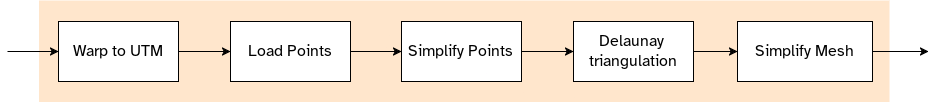
\includegraphics[width=1\textwidth]{assets/meshConstruction-zoomed.png}
  \caption{Flow graph showing the process required to generate a mesh from DEM data}\label{fig:meshConstruction:dataprocessing}
\end{figure}

\autoref{fig:meshConstruction:dataprocessing} outlines the pipeline from initial WGS84 DEM dataset to Delaunay Triangulation. The choice to simplify the point-set before triangulation, and again simplify the mesh after simplification was designed to allow for an exploration into performance differences and tweaks to the simplification, which are discussed later (see \autoref{section:impl:meshProcessing}.).

\subsection{Data Feature Representation}\label{section:design:mesh:dataFeatures}

Due to the limitations of W. Evans' approach of constructing the search graph solely using topography data, this project developed a novel approach to more accurately represent feature data within the search graph.

Two types of features were identified: area features, and edge features. When traversing over an edge, some features relate more to the surface (i.e. terrain area) being traversed; whereas others relate to the path itself (i.e. edge). For example, terrain type is best categorized as an area feature, as its volume over the surface is meaningful. Paths, however, are often best represented as edge features, as their width is often is irrelevant to travel on-foot.

The approach to representing these features accurately is similar but requires slightly different setup. Overall, the process aims to apply the geometry of both types of features as constraints in the Delaunay triangulation.

For edge features, adding a constraint onto the mesh ensures that edge exists in the final mesh. For area features, we can ensure that feature tagging can be done accurately by applying the edges of data into the mesh as constraints. This ensures borders of data are enforced, improving the resolution of routing decisions, as accurately following the borders of features is possible.

These constraints are added based on the $X,Y$ coordinates of the contours, and are placed at the relevant $Z$ coordinate on the original mesh to prevent unwanted changes to the topography.

This method is likely sufficient for most data features whose data refers to regions of the terrain (e.g. paths, terrain types, building positions, etc.). Some notable 3D data features that cannot be represented however are: heights of bridges, which may be relevant due to the fear-of-height response; and the height of objects which may be climbable (although legal restrictions usually prevent climbing over objects captured in GIS datasets).

\subsubsection{Vector Features}

Vector data is directly represented in the search graph using constraints in the Delaunay triangulation. For example, fetching the geometry of paths enables constraints to be applied corresponding to the individual edges in the contours of paths. This enables a high accuracy representation of vector features.

\subsubsection{Raster Features}

\begin{figure}[H]
  \centering
  \subfloat[CEH Terrain Data]{
    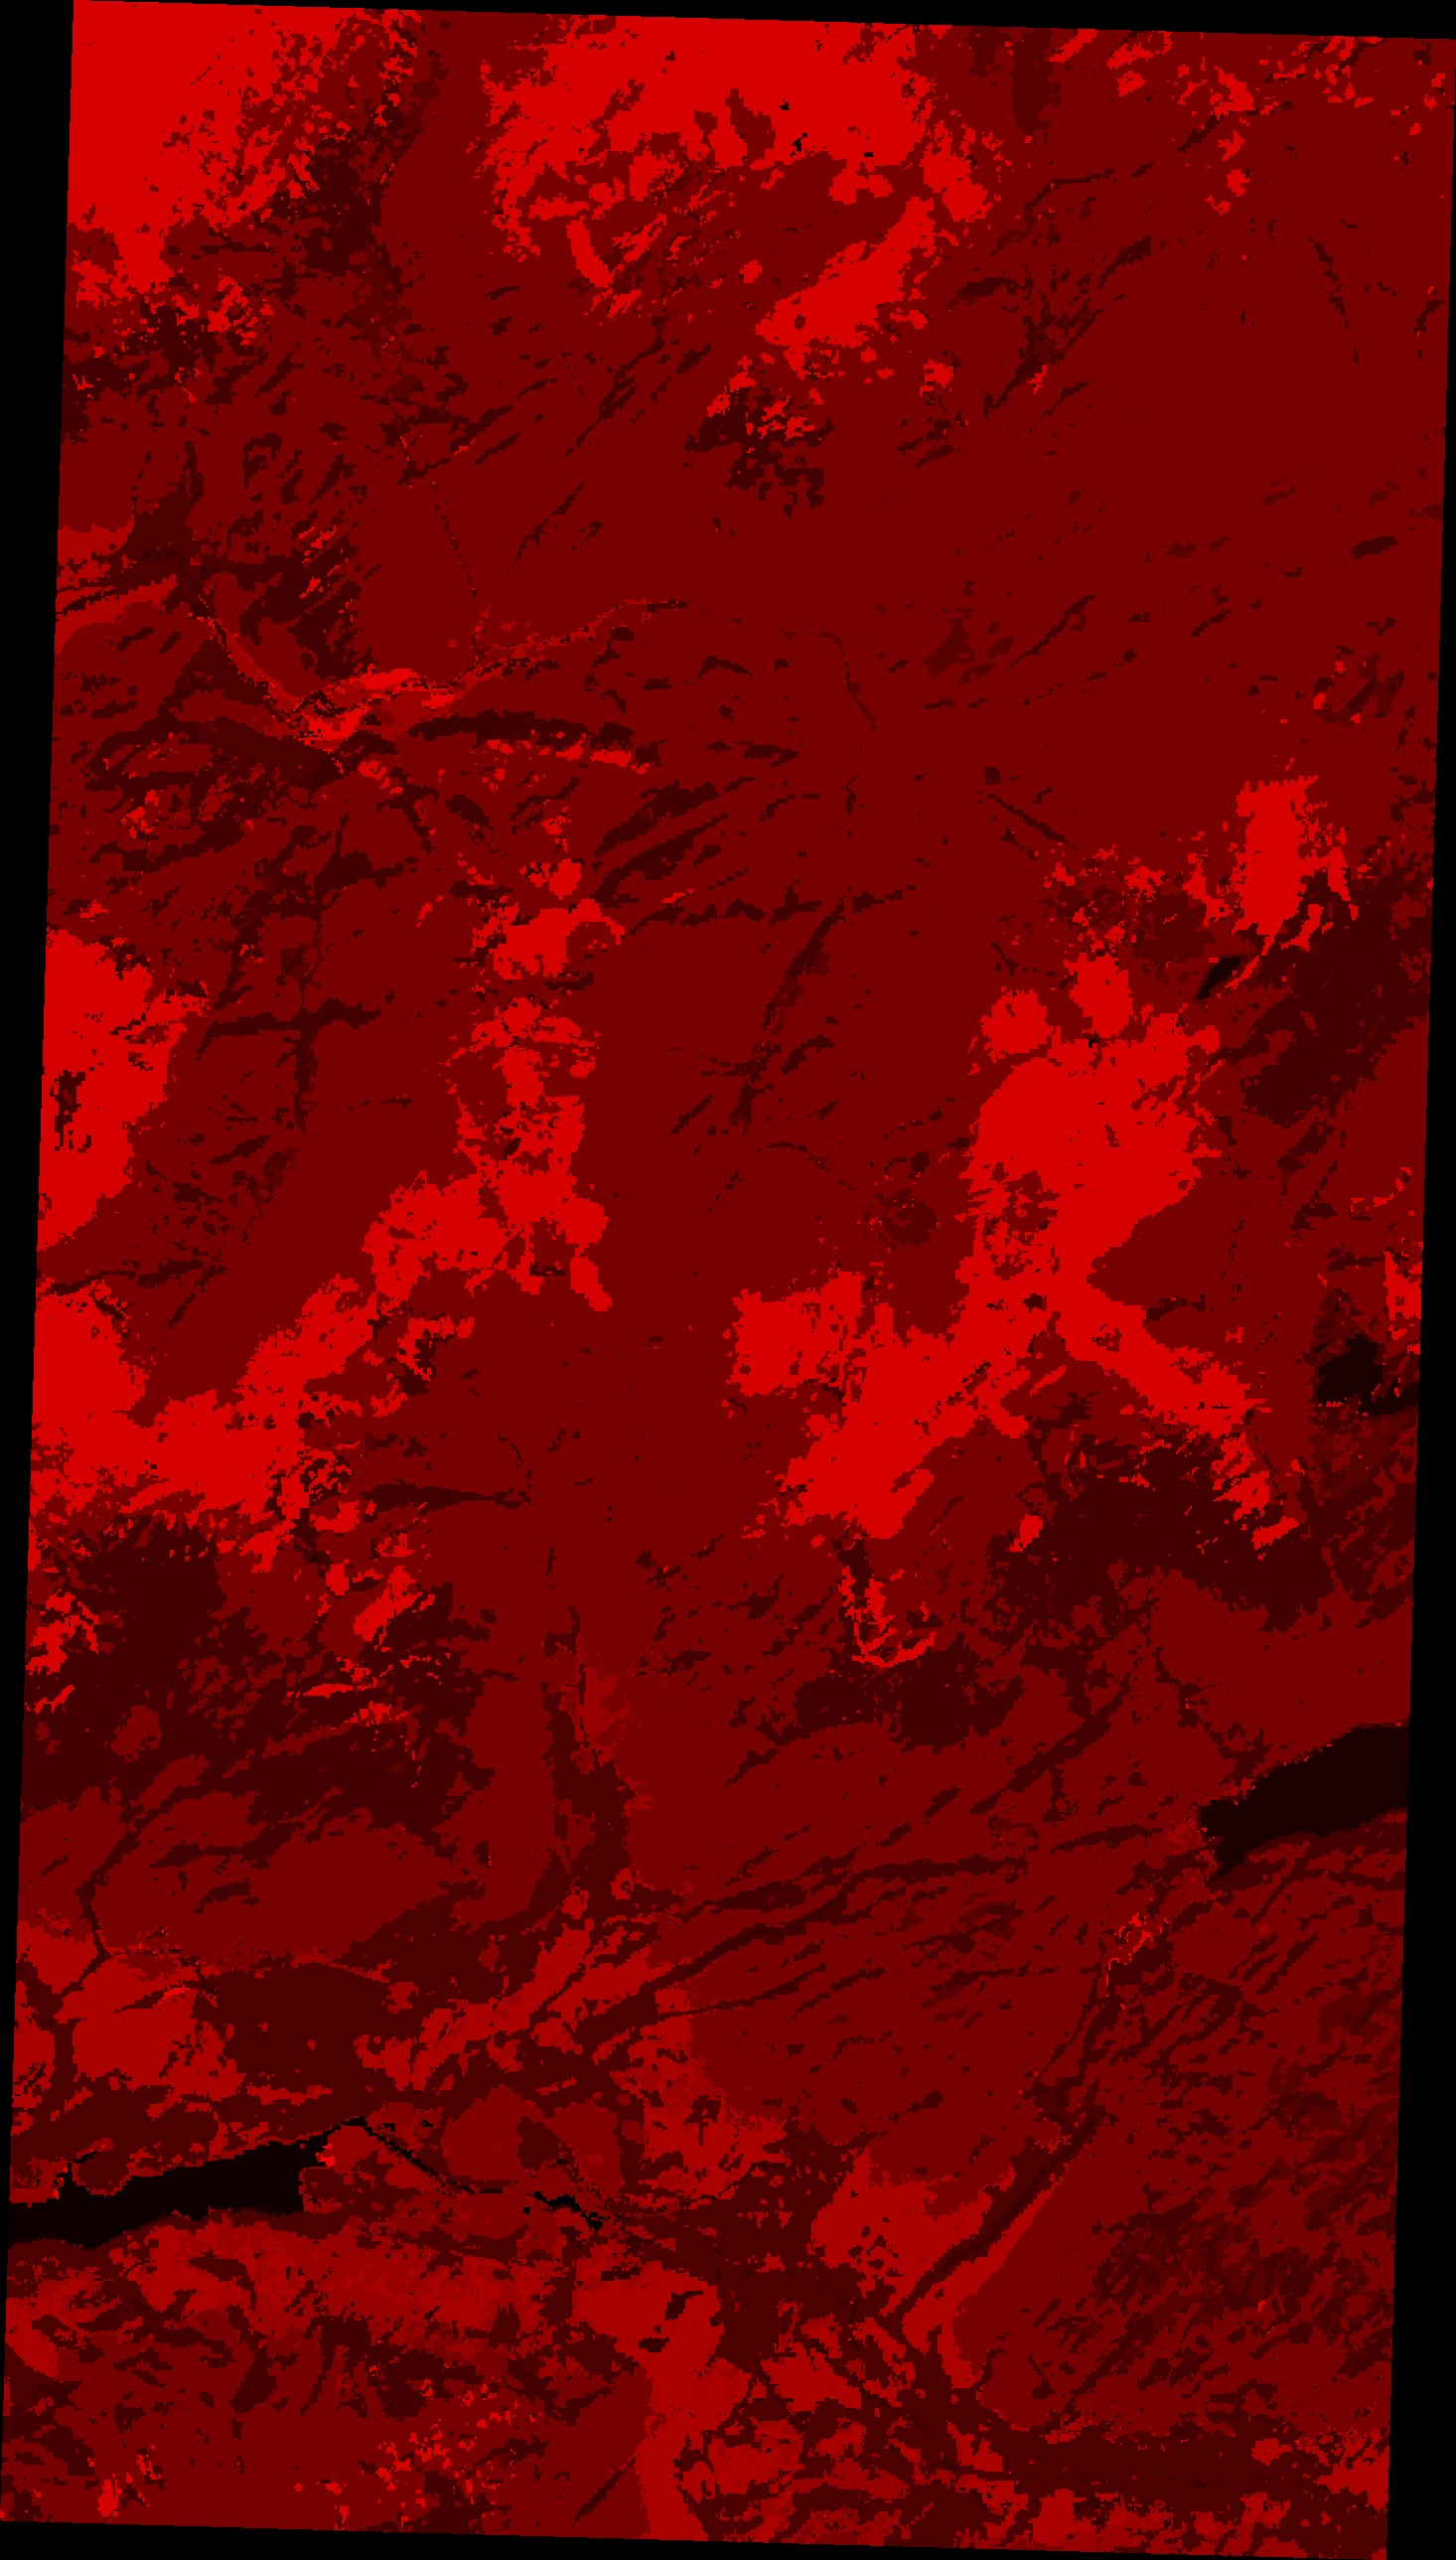
\includegraphics[width=0.35\textwidth]{assets/benNevis-chunk-terrain.png}
  }
  \subfloat[Detected Edges of the CEH Terrain Data] {
    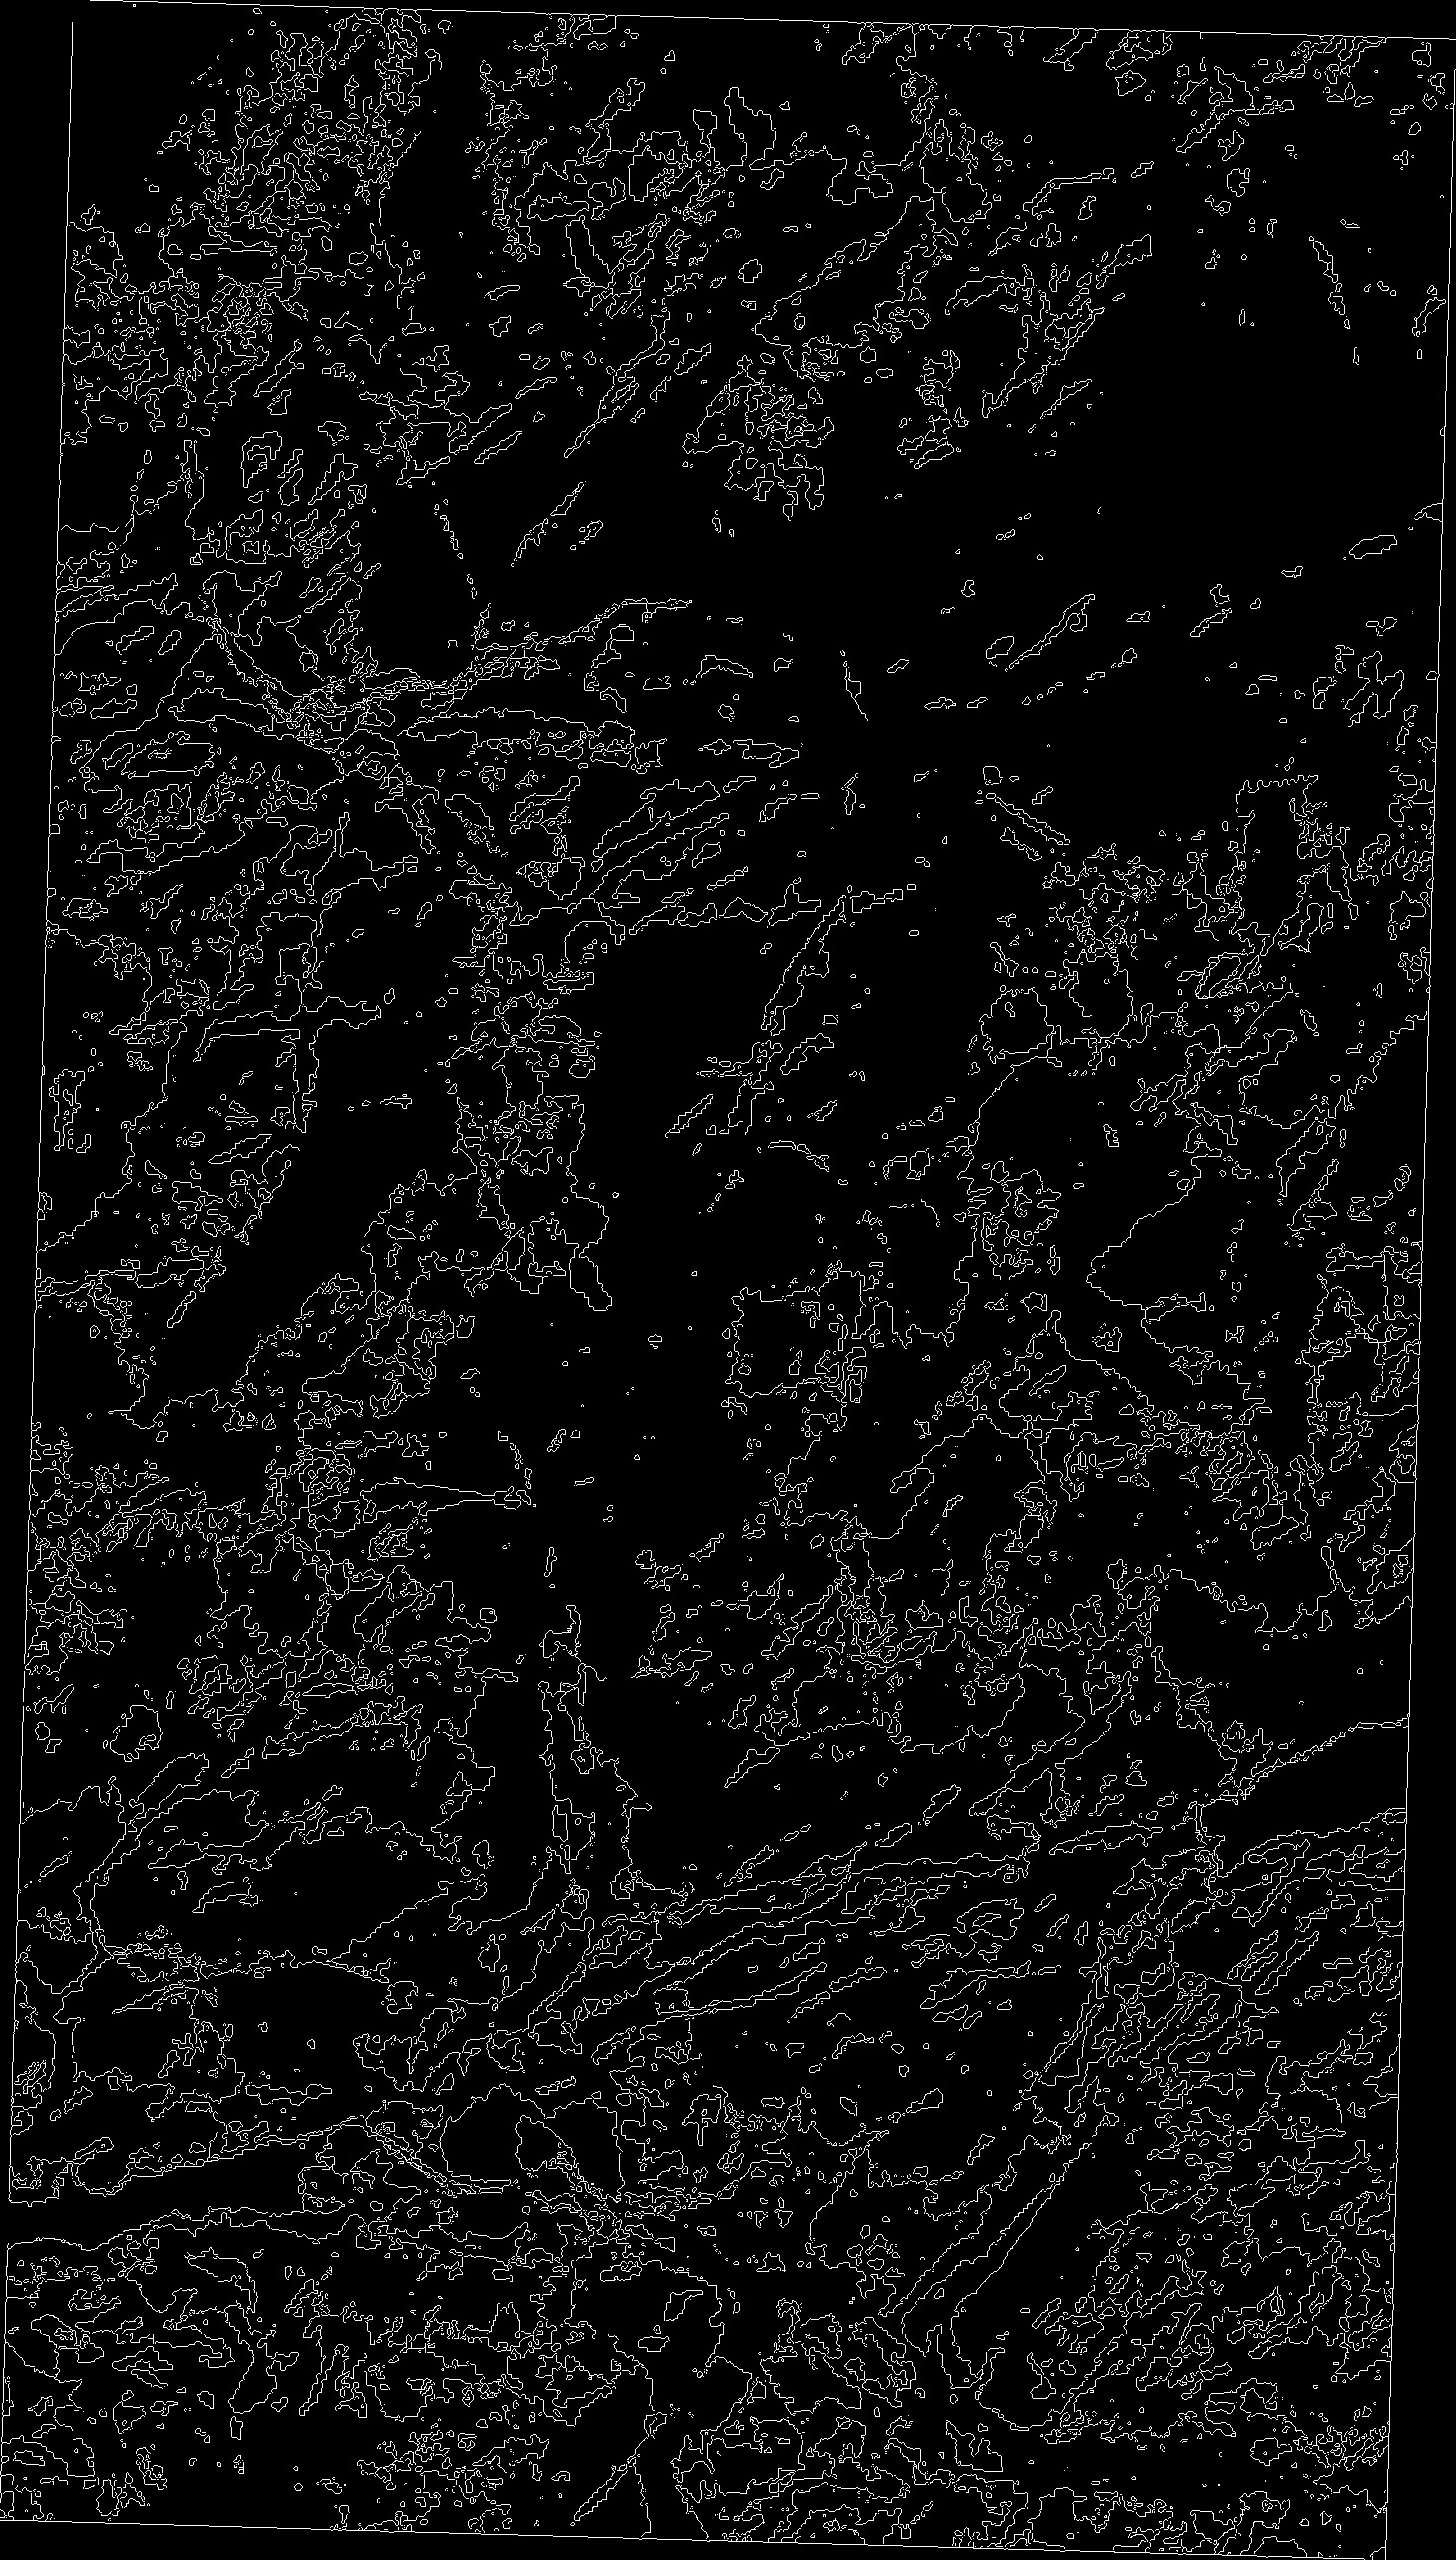
\includegraphics[width=0.35\textwidth]{assets/benNevis-chunk-edges.png}
  }
  \caption{The edges detected from a chunk of terrain-type data warped to UTM.}\label{fig:edges:terrain}
\end{figure}

Computer vision enables vector edges to be detected and extracted from raster data, which can then be converted into a set of constraints that can be applied onto the mesh.

Applying data edges as constraints is sufficient to accurately represent feature locations. \autoref{fig:edges:terrain} shows the detected contours along with the original terrain type data. Every region defined by the contours have a uniform terrain type. Constraints ensure that edges fully cover each data border, and so every triangle will fall within, and not overlap any, terrain section --- getting the pixel value for any point in these triangles will therefore give the correct terrain type. Using constraints to define data borders enables a high accuracy dataset to be represented even on a low DEM resolution mesh.

\subsection{Routing Algorithm}

The actual routing algorithm is a uniform-cost-search algorithm, searching on the vertices of the TIN. It aims to find the minimum-cost path from a given start point, to a given end point, given a cost function and search boundary. The cost function is outlined in the next section, but is constructed to the Features mentioned previously.

The algorithm works through the accumulation of non-negative costs from the start node. The costs are calculated per edge in the graph (from one point to another), and stored in a priority queue, enabling the algorithm to search the lowest-cost routes first. The process of searching follows the repetition of a three-step loop:

\begin{enumerate}
  \item Check exit conditions

        The exit condition is satisfied once the minimum accumulated cost for the target node is found. This means routing to and from the same point will be handled gracefully by exiting immediately.

  \item Select Next Node

        We begin by selecting the source node with zero cost (as it costs nothing to travel nowhere). From there, we select the node pointed to by the minimum accumulated cost in our priority queue. That node's minimum cost is set to that edge's accumulated cost value.

  \item Search Adjacent Unsearched Nodes

        For each connected edge that points to a node that doesn't already have a minimum cost set, we calculate the cost to get from the current node to that node, and add that cost to the priority queue.

\end{enumerate}

Once exit conditions are met, we reconstruct the route back from the target node to the source node. From the target node, we fetch its minimum cost, and follow the edge that lead to that minimum cost to the previous node. We fetch its minimum cost, and continue following back until the source node is reached.

This uniform cost search means that nodes that have a minimum cost to reach, higher than that of our target node are never searched.

\subsubsection{Search Boundary}

Defining a search boundary reduces both the amount of data that is required to be downloaded from APIs, and loaded into memory during search. \textcite{evans2023tsr} discusses the issues from using a standard bounding-box like approach such as searches with a similar latitude or longitude value will have a very thin bounding box, limiting the ability to search potential routes. Instead, a rotated bounding box is defined, calculating the distance between the two points, and drawing circles around the points with a radius equal to some proportion of their distance, a rotated rectangle border is then drawn connecting these circles. This approach tends towards a wider search radius for long-distance searches,  and narrower search radius for short-distance routes as the further a user needs to travel, the more likely an obstacle is to exist within a certain search width.

\subsection{Cost Function}

\begin{figure}[H]
  \centering
  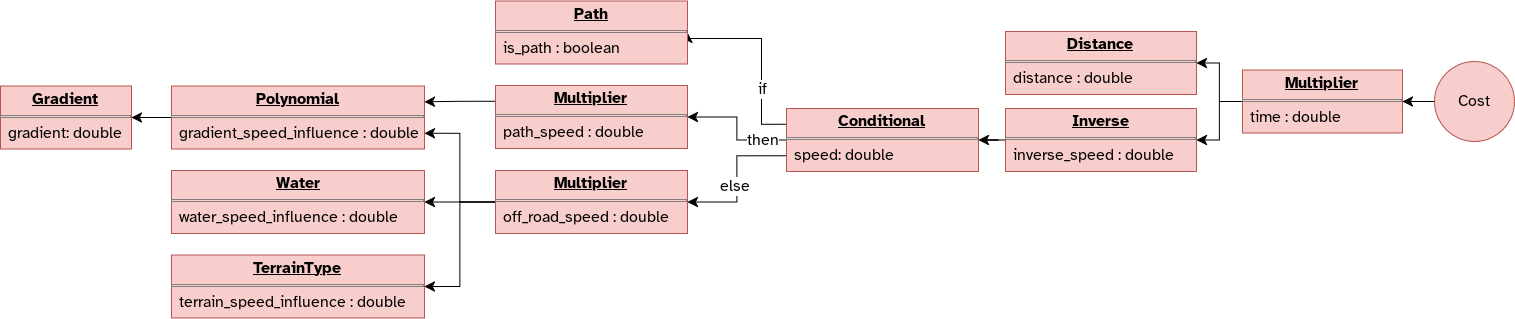
\includegraphics[width=\textwidth]{assets/costfunction-example1.png}
  \caption{Example DAG cost function design. Output models an estimated travel time using three factors influencing travel speed.}\label{fig:cost:example:1}
\end{figure}

A primary contribution this project has made is with the design of the cost function. The cost function is represented as a directed acyclic graph (DAG) of features. Each feature outputs a single value. Connections between features allows the output of one feature to be used as an input to another feature forming dependencies. Features may have any output type, but the dependency input/output types must match, and the final output feature may be any number producing feature. This flexibility allows future development and experimentation of cost features.


\autoref{fig:cost:example:1} demonstrates the capacity for the cost function to model mathematical functions. Here, the default cost function is given, which models a value directly proportional to time:

\[\frac{\text{Time}}{\text{Default Walking Speed}} = \frac{\text{Distance}}{\text{Speed Influence}} = \text{Distance} \times \frac{1}{\text{Speed Influence}}\]

The default speed refers to the default walking speed on a flat road surface in meters per second. We don't actually need this value to calculate the cost, as it is constant, and so the resulting costs can be converted into estimated time by dividing the final cost by this value giving travel duration in seconds. This value can be changed to model a specific users average walking speed, but defaults to the pace defined in the FHWUA's Manual on Uniform Traffic Control used to define how long pelican crossings should allow for walking --- 1.2 meters per second \autocite{united1978manual}. We can then calculate the speed influence, referring to how much slower/faster than the default speed walking over this edge is.

\subsection{Features}

\begin{figure}[H]
  \centering
  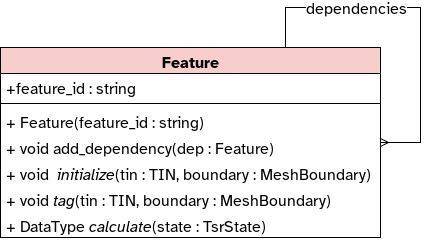
\includegraphics[width=0.5\textwidth]{assets/feature.png}
  \caption{Feature class UML design.}\label{fig:feature}
\end{figure}

Features are designed to be able to represent any data or mathematical concept. Some features are categorical, numeric, or informational. Therefore, features have been designed to be able to output any data type. \autoref{fig:feature} shows the design of a basic feature. Features are designed to use other feature's output as input, and so the output types must match expected dependency types. In addition, the final cost output feature must output a number value representing the cost. This allows complex data relationships to be modelled modularly, which makes re-using components in different configurations easier as the data can be outputted in its original type, with different interpreter features used to model different factors related to that data.

\subsubsection{Features Setup}

\begin{figure}[H]
  \centering
  \subfloat[Initialization] {
    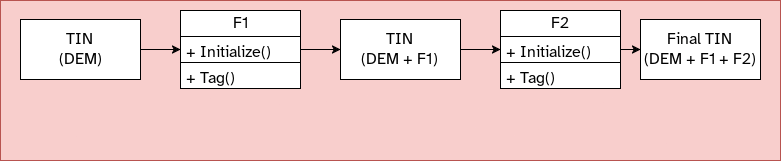
\includegraphics[width=0.45\textwidth]{assets/FeatureSetup-Initialize.png}
  }
  \subfloat[Tagging] {
    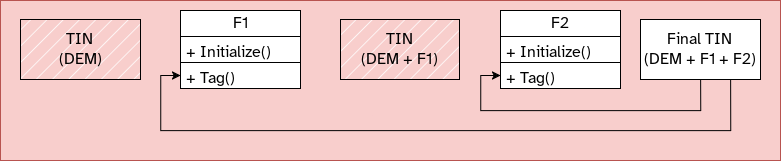
\includegraphics[width=0.45\textwidth]{assets/FeatureSetup-Tag.png}
  }
  \caption{Initialization and tagging phases of feature setup. Showing how features interact with, and modify the TIN search mesh.}
  \label{fig:design:features:setup}
\end{figure}

Each feature follows the same three-step setup process: configuration allowing users to define option values; initialization of the feature, which may modify the search graph as described in \autoref{section:design:mesh:dataFeatures}; and finally tagging.

Features by default set in the first stage just a unique identifier, which is used to check for dependency cycles in the cost function. Features may add configuration options to this construction. This allows user-preferences to be defined, benefiting the accessibility of the final product such as the degree to which paths are preferred over off-road terrain. These configuration options also enable data simplification and processing options to be modified, making it easier to test different processing options in testing.

The initialization and tagging stages of the setup process are outlined in \autoref{fig:design:features:setup}. The initialization stage is designed to allow for features to prepare data if required, and add contours to the TIN. The tagging stage is designed to enable caching of data results to improve performance during cost-calculations. For example, it is more performant to open a dataset once and tag each face with the terrain type, than to open and close the file each time a cost is evaluated. However, tagging would be invalidated if the TIN is modified, hence why tagging must be done separately to initialization, so that all features can add contours to the TIN before tagging takes place.

\subsubsection{Data vs Logic Features}

Whilst all feature types are treated the same, it is useful to distinguish data features, with logic features. Logic features take input, apply some logic, and output the value. Data features use datasets to give information about some feature of the terrain.

Every data feature will require a very similar design to their initialization and tagging setup functions.

For initialization, the example data features, and likely most data features, will fetch the required area of data for the given search area. Then, if required, contours will be extracted from that data feature and applied onto the mesh. Additionally, any caching of information that is not related to components of the mesh itself can be stored in initialization, as other features may manipulate the mesh further. Tagging enables mesh-specific data to be related in feature attributes.

Logic features on the other hand likely require little initialization or tagging. Examples such as gradient and distance are best calculated during routing, as the gradient and distance for a search edge is likely only useful for when that edge itself is having its cost calculated. This reduces overall computation when uniform cost search skips nodes once the target node is found.

However, these distinctions are conceptual only, and features are welcome to put any logic in any of the three core setup and calculation logic, as long as the TIN is only manipulated in the initialization stage. Following with include the specific design of some primary example features constructed.

\subsubsection{Multiplier Feature}

The multiplier feature enables concepts such as speed and time to be created using a mathematical model of the concept. For example, speed is calculated as the multiplication of a number of given speed influences.

\subsubsection{Gradient Speed Feature}

To use the gradient to model speed, the raw gradient value must be converted into some factor that is multiplied to the speed, suggesting the relative slow-down/speed-up factor from the gradient. To support customization, the design of this feature enables a polynomial of any degree to be inputted. The default values are constructed using results from \autocite{horiuchi2015comparisons}, and applying a polynomial regression algorithm to get a polynomial line of best fit. This approach is efficient for cost-evaluation, as fetching the speed influence value is completed by solving the polynomial equation, and clamping negative speeds to 0. An alternative design would be Bézier curves which would enable custom curves to be defined by creating and moving points manually --- this approach may still be an interesting further development as it would make customization easier as an interactive UI could be developed. However, as gradient calculations are required for each edge, more complex Bézier curves require more computation to solve for $y$.

\subsection{Graph Traversal}

Dijkstra's algorithm was selected to serve as the basis of this search algorithm. Specifically, uniform cost search, as the ultimate goal is to find the optimal route between two nodes. Uniform cost has lower space complexity due to the storage of a best-cost only once the node has been searched, unlike Dijkstra's initial design which requires setting all nodes to infinity best-cost initially.

\subsection{API}

Constructing both the initial topographical TIN and setting up data features require datasets from online APIs. Given a search, this application is designed to automatically fetch the GIS data required. These APIs have different, yet similar formats, and designing a simple interface that can be customized to work for any API format makes adding new features easier. Having automatic fetching of data from APIs is important for the user-experience and accessibility of the application, as otherwise each dataset would have to be manually downloaded and given to the application in some way.

\subsection{Chunking}

\begin{figure}[H]
  \centering
  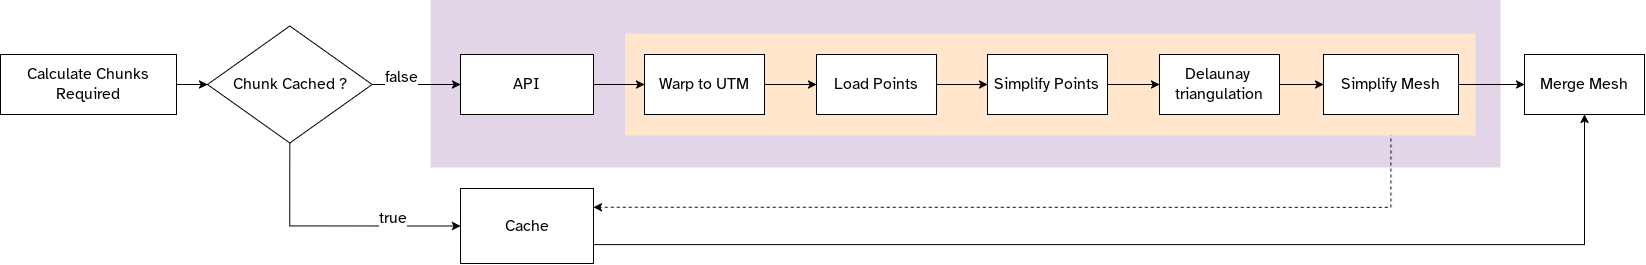
\includegraphics[width=1\textwidth]{assets/meshConstruction.png}
  \caption{Final search graph construction process with automatic chunking, API calling, and caching.}\label{fig:meshConstruction:full}
\end{figure}

For extensive searches, the system efficiently handles large volumes of Digital Elevation Model (DEM) and feature data by dividing it into manageable square tiles of a specified size. This method, known as chunking, ensures that data is loaded and processed safely while maintaining consistent partitioning across different uses of the application.

By automatically dividing land into uniform tiles, the system optimizes API calls and caching. This reduces the number of requests and processing required for subsequent searches, improving both speed and efficiency. Entire tiles are downloaded and processed, including those overlapping the search boundary, allowing complete caching of these tiles for future use.

This approach minimizes redundant data retrieval, accelerates operations, and ensures seamless handling of large datasets. It not only enhances performance but also reduces computational and network resource demands, making the system robust and scalable.

\subsubsection{Parallelism}

\begin{figure}[H]
  \centering
  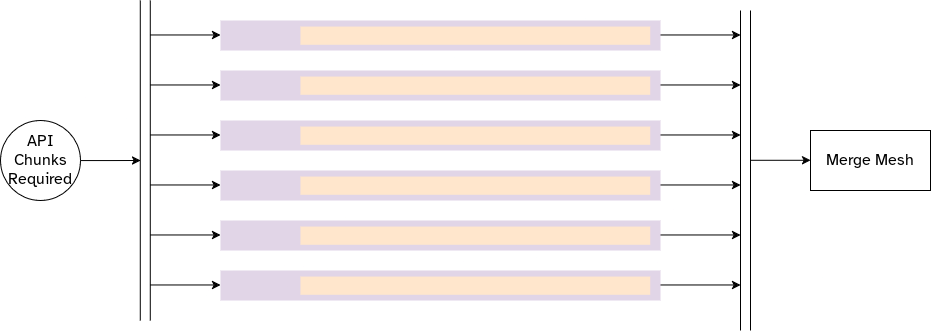
\includegraphics[width=1\textwidth]{assets/meshConstruction-parallel.png}
  \caption{Parallel design of processing DEM chunks into a completed TIN.}
  \label{fig:meshConstruction:thread}
\end{figure}

After determining required chunks, data is fetched from the API (see. \autoref{fig:meshConstruction:full}). Each chunk is fetched, processed, and stored, completely independently of each other. This enables parallelization of this process --- spawning threads for each chunk. To prevent too many processes using similar resources (network, storage, etc.), a pipeline structure is used, allowing a certain number of threads to be created for each stage --- this is shown in \autoref{fig:meshConstruction:thread}.


\subsubsection{Caching}

In addition to enabling parallelization, the independence of chunk processing and storage enables useful caching. Caching enables different searches to use data from previous searches. If two searches have overlapping search areas, the overlapping data can be re-used between calls. By processing and caching entire chunks of data, we can check which tiles are  cached, and fetch them, requiring only limited processing to remove out-of-bounds points and reconstruction. As tiles are uniformly aligned, alignment is easy as we know exactly where each tile starts and ends. This reduces the number of API calls required, dramatically improving setup performance where cached data is used.

\section{Implementation}

This section discusses some specific challenges encountered, and the solutions developed during the implementation of the design of this route planner.

An important note: UML diagrams are used to represent C++ classes. Pointers are shown with asterisks (e.g. \texttt{Feature *}). Where used, and unless otherwise specified, these refer to smart pointers. Smart pointers give far better memory safety, as objects are automatically freed from memory when out-of-scope, preventing the need to remember to manually free objects which easily leads to memory leaks if omitted.

\subsection{Output Visualization}

The route planner generates KML files as output for use with Google Earth. A path is drawn between the source point and end point, following the recommended route given by the router. Colours are applied from green to red representing the gradient difficulty.

Where applicable, warnings are displayed telling users of potential hazards in the surrounding area, giving a brief description and estimated location. This gives insights into the reasons routes were chosen over others, and increases the safety, as users are aware of specific features to avoid. To improve readability, only warnings for areas close to the generated route are displayed, which are likely the only warnings relevant when following the route. Additionally, when debugging, features generate KML files displaying the stored information such as which faces contain water, or do not have a value applied. When no safe route can be found, all warnings generated during routing are displayed. This gives insight into where barriers exist, and how much of the graph was searched which is helpful for debugging.

In addition, the gradients of sections of the route are suggested using the colour of the route, spanning from red to green, with red representing more difficult gradients (positive and negative gradients), and green representing easier to traverse gradients.

\subsection{Mesh Derivation}

CGAL was used for converting the DEMs to TINs. CGAL offers constrained Delaunay triangulation, which is an essential design feature of the mesh. In addition, to enable initial experimentation with mesh optimization, CGAL does not impose a limit to the number of components in the mesh like the Fade library.

% CGAL's constrained Delaunay triangulation is done automatically by the \texttt{Constrained\_\allowbreak Delauany\_\allowbreak Triangulation\_2} class. CGAL enables 2.5D triangulation through this class, with the addition of the \texttt{Projection\_\allowbreak Traits\_\allowbreak \_xy\_3}. This triangulates points on the $xy$ plane, and then applies the $z$ position onto those points.

This 2D Delaunay triangulation projected onto 3D is less complex than using a 3D Delaunay triangulation, which constructs tetrahedra. \textcite{perkins2013fielddstar} found that routing over tetrahedra is also less performant. In addition, the DEM data used is 2.5D, and so little benefit would be gained from a 3D triangulation.

\subsection{Mesh Processing}\label{section:impl:meshProcessing}

The initial implementation triangulated the raw DEM data with no pre-processing to remove the number of points. Performance quickly became an issue for reasonably small search distances, due to the fact that 30m resolution DEM data includes 2916 points per square mile.

Two forms of simplification were implemented: pre-processing the DEM point set, and processing the constructed mesh itself. Both use CGAL's tools for this process. Both processing steps must be done before features are initialized, as they are likely to impact the accuracy of contours added. This two-step processing enabled experimentation of different approaches, as research on CGAL's implementations has not been conducted. Further experimentation would benefit the accuracy of the resulting mesh, as some finer details are affected by the processing implemented.

\subsubsection{Point Set Pre-Processing}

To simplify the point set, the \texttt{hierarchy\_simplify\_point\_set} function is used --- allowing the setting of the maximum size and maximum variation of clusters, and groups points into clusters of a given size, and removes vertices that are within the maximum variation bound set. In addition, the \texttt{wlop\_simplify\_and\_regularize\_point\_set} tool was used, which supports parallelization out of the box, allowing configuration of the maximum percentage of points that can be removed, and the closeness of similar points that can be flattened into a single point.

Extensive visual experimentation was done to find settings that maintained the visual accuracy of the topography. The final result reduces the overall mesh size by an average of 60\%.

Initial simplification of the point set provides far better performance than simplification of the mesh. This is due to the Delaunay triangulation also seeing performance gains from the reduction of points. In addition, the simplification itself is more performant on the point set as the mesh must maintain the features of the mesh (i.e. edges, faces, etc.) when the mesh is updated. However, CGAL only offer simplification of almost-planar patches on meshes, and not point sets.

\subsubsection{Mesh Processing}

The mesh simplification tool used for this project was initially the \texttt{remesh\_almost\_planar\_patches} utility which allows sharp edges to be detected and protected, and almost planar (almost flat) regions to be using parallelization if supported. However, the performance was still relatively poor, and mesh integrity issues have been documented. Further developments to this tool may be useful for this project, as this tool does not impact finer details as much as the point-processing method.

What is implemented in the final submission are simple removal of invalid elements, and the removal of duplicate vertices.

\subsection{Features}

\begin{figure}[H]
  \centering
  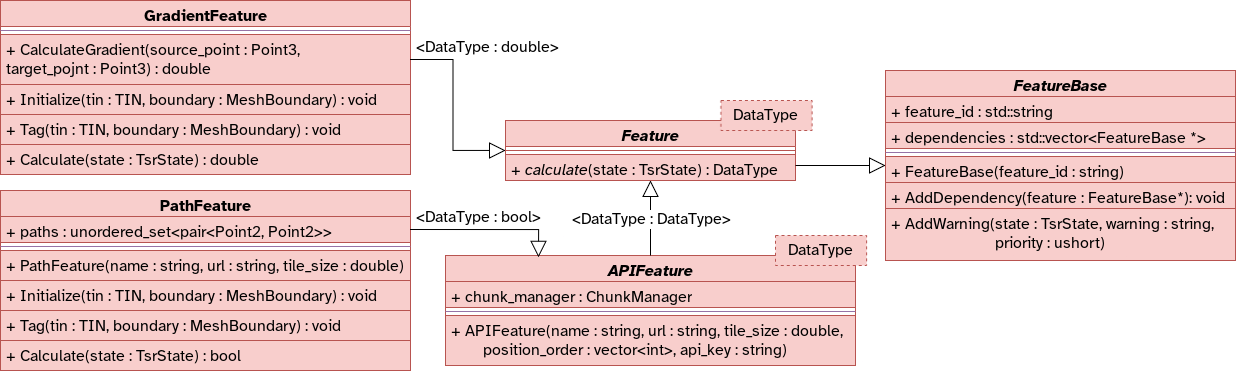
\includegraphics[width=\textwidth]{assets/FeatureBase.png}
  \caption{UML diagram showing the basic \texttt{FeatureBase} and Feature interfaces, with the specialized \texttt{DataFeature} interface, and two example of actual Features that can be instantiated.}\label{impl:features:uml}
\end{figure}

\subsubsection{Setup}

The \texttt{initialize} and \texttt{tag} methods are abstract/virtual, meaning each feature must define their own methods following this template. This allows features to implement empty methods if no configuration is required, such as a purely mathematical feature such as the gradient or distance features, or call APIs and cache results such as with the \texttt{PathFeature}, \texttt{WaterFeature}, and \texttt{CEHTerrainFeature}.

\subsubsection{Dependencies}

Features communicate through dependencies, and define the DAG cost function structure. By default, the \texttt{add\_dependency} functionality inherited by all features adds the pointer to the dependency to the \texttt{dependencies} vector. This means that the order dependencies are added is essential to fetching the results. For example, the \texttt{ConditionalFeature} requires the conditional dependency to be added first, then the true condition, and finally the false condition. Dependencies will often use a \texttt{DEPENDENCIES} enum internally to give names to this order to make code easier to read (see \autoref{fig:conditional} for an example).

\subsection{Raster Feature Edge Detection}

As mentioned in the design section, raster area features use computer vision to detect the edges and convert them to vector contours. The edge detection itself is handled by the OpenCV library, offering canny edge detection, which detects sharp changes in values (i.e. data borders), which are then converted to a vector of vectors of points representing the contours which are just vectors of points.

\subsection{Data Position Alignment}

The position of data points within any GIS dataset is essential to accurately extract when relating the data to our mesh.

Aligning vector data is straight forward, as each point is defined with a coordinate position in whatever coordinate system is used. As discussed, these datasets can be warped as points are extracted, or preprocessed as done in this implementation with GDAL --- this was chosen to maintain a similar workflow to both vector and raster dataset processing.

Raster data required more configuration to align. As raster datasets are ultimately images, data is given in a grid of pixels, where each grid position just gives the value. Metadata in raster GIS datasets allows the coordinate of each pixel to be calculated with this calculation:

\begin{align}
   & x = \text{upper left x} + \text{pixel width} \cdot \text{pixel x} + \text{row rotation} \cdot \text{pixel y}     \\
   & y = \text{upper left y} + \text{column rotation} \cdot \text{pixel x} + \text{pixel height} \cdot \text{pixel y}
\end{align}

This formula is also useful for applying extracted contours to the TIN, as they are extracted with coordinates relative to the image dimensions and origin.

\subsection{Data Features}

Data features are those features which require the use of API or local data sources. This includes: water data, path/road data, and terrain type data. The \texttt{DataFeature} abstract class is designed to support the construction of new data feature classes, adding a \texttt{ChunkManager} attribute, which enables automatic fetching of required chunks from the API and caching --- making extension of this project with new data simpler.

\begin{figure}[H]
  \centering
  \begin{lstlisting}[language=c++]
	class ChunkManager {
		std::string url;
	
		double tile_size;
		std::string api_key;
		std::vector<int> position_order;
	
	public:
		ChunkManager(std::string url, double tile_size,
								 std::vector<int> position_order, std::string api_key)
				: url(url), tile_size(tile_size), api_key(api_key),
					position_order(position_order) {}

		std::vector<ChunkInfo> GetRequiredChunks(const MeshBoundary &boundary) const;

		ChunkInfo GetChunkInfo(double lat, double lng) const;
		std::string FormatUrl(const ChunkInfo &chunk) const;
	
		DataFile FetchVectorChunk(const ChunkInfo &chunk) const;
		DataFile FetchAndRasterizeVectorChunk(const ChunkInfo &chunk,
		DataFile FetchRasterChunk(const ChunkInfo &chunk) const;

		bool IsAvailableInCache(const std::string &feature_id,
														const ChunkInfo &chunk);
	};
	\end{lstlisting}
  \caption{\texttt{ChunkManager} class, which enables easy setup and interface for Data Features to  interact the API/cache.}
  \label{lst:chunkmanager}
\end{figure}

Different features can define a tile size, allowing datasets with varying resolutions to be handled efficiently, without requesting too much or too little data in one chunk. Each tile chunk is represented by the latitude and longitude coordinates of its southwestern and northeastern corners in the WGS84 projection --- the standard projection for GIS datasets. The southwestern tile position is determined by rounding the latitude and longitude values down to a multiple of the tile size. By adding the tile size to these values, we get the northeastern corner.

The \texttt{ChunkManager} is setup by the \texttt{DataFeature} object with a URL specifying the location of the API to fetch data from. GIS API endpoints usually function throughout the specification of the resource, with a bounding box given in latitude and longitude coordinates: the \texttt{position\_order} vector in \autoref{lst:chunkmanager} is used to specify the order of the minimum and maximum latitude and longitude values. Some APIs (e.g. OpenStreetMap's Overpass API) enable fetching of multiple data types in one request, and so the \texttt{url} contains \texttt{\{\}} representing values replacements, with the coordinate specified in the \texttt{position\_order} vector. This standard makes it simple to introduce new and more complex API data features.

\subsubsection{Water Feature}

\begin{figure}[H]
  \centering
  \begin{lstlisting}
	https://lz4.overpass-api.de/api/interpreter?data=
	[out:xml][timeout:25];
	(nwr["natural"="bay"]({},{},{},{});
	nwr["natural"="water"]({},{},{},{});
	nwr["natural"="coastline"]({},{},{},{});
	);
	(._;>;);
	out body;{}
	\end{lstlisting}
  \caption{Decoded and formatted URL used to fetch the water data from the OpenStreetMap Overpass API.}
  \label{url:water}
\end{figure}

OpenStreetMap (OSM) data was chosen to fetch water features due to its higher resolution compared to the terrain type data from CEH. OSM represents features in vector format; giving very high positional resolution. These edges could be directly added as contours to the mesh. However, certain water features such as coastal barriers, and small streams are represented as lines with no geometry, making it challenging to determine which side of the line has water.

It may be possible in future research to use the fact that the ordering of coastal and lakes edges follows the right-hand rule, where following the order implies the right-hand side is filled with water. However, rasterization is used to simplify the tagging process, as the relevant pixel values can be fetched from the datasets.

OpenCV edge detection is used on the rasterized dataset to re-fetch data edges. This ensures that any rasterization resolution changes are reflected in the contours applied to the mesh. Otherwise, additional contours may be applied erroneously, as the faces would be tagged incorrectly due to the pixel values in the raster dataset being incorrect.

\autoref{url:water} gives the URL format used for this \texttt{DataFeature}. OSM offers three categories of water features with geometry which are all fetched. No API key is required.

\subsubsection{Path Feature}

\begin{figure}[H]
  \centering
  \begin{lstlisting}
	https://lz4.overpass-api.de/api/data=
	[out:xml][timeout:25];
	(
		way["highway"]({},{},{},{});
	);
	(._;>;);
	out+body
	{}
	\end{lstlisting}
  \caption{Decoded and formatted URL used to fetch the paths and roads from the Overpass API.}
  \label{url:paths}
\end{figure}

OpenStreetMap data was also used to fetch paths and roads. These vector edges are directly applied to the mesh. \autoref{url:paths} shows the URL used, which fetches all roads and paths in one request.

This returns an XML dataset with the geometry of each road, along with a vast amount of metadata for each path/road. This data could be greatly useful in further developments (see. \autoref{section:improvements:paths}).

The XML data is converted to GeoJSON during warping using a JSON parser. This functionality is added as it enables new vector features to use JSON without additional library requirements, and reduces the likelihood of bugs in code fundamentally tangential to the aims and objectives of this project.

These paths are then stored as points in a \texttt{map} of road segments as coordinate pairs. This enables checking if the current edge's vertices match the location of a road segment, which is done in $\mathcal{O} (1)$ time regarding the number of path segments added. In urban areas, this number is potentially extremely large as geometry of the roads is represented, and so this performance characteristic is essential.

\subsubsection{CEH Terrain Type Feature}

\begin{figure}[H]
  \centering
  \begin{lstlisting}
	https://catalogue.ceh.ac.uk/maps/4728dd2d-064f-4532-be85-ecafc283bdcf?language=eng
	&SERVICE=WMS&VERSION=1.3.0&REQUEST=GetMap
	&CRS=CRS:84&LAYERS=LC.10m.GB&STYLE=default
	&BBOX={},{},{},{}
	&FORMAT=image/tiff
	&WIDTH=2048&HEIGHT=2048{}";
	\end{lstlisting}
  \caption{Decoded and formatted URL used to fetch the terrain type data from the CEH API.}
  \label{api:terrain}
\end{figure}

The raster terrain data from the Centre for Ecology and Hydrology (CEH) was used as it offers a diverse categorization of the land-use of terrains in a raster image. The edge detection is used to fetch the boundaries for this data. A challenge for this was in detecting the borders between the RGB values which are represented each as their own layer in the dataset files.

The simplest method to fetching each contour between colours in each band would be to run the detection in each band separately, and then combine the edges. This is successful, but results in duplicate edges in areas where differences exist between colours in two or more of the RGB channels. To remove the need to process these edges after edge detection, and to reduce the processing requirements, the images can be converted to greyscale. This solves the previous issues, but greyscale fails to result in edges being detected where the contrast/brightness of two colours is not great enough. For this dataset in particular, this issue was not encountered, but further development may require more complex processes to extract multilayer contours using computer vision.

\begin{figure}[H]
  \centering
  \begin{lstlisting}[language=c++]
	std::map<uint32_t, CEH_TERRAIN_TYPE> CEHTerrainFeature::TERRAIN_COLOURS = {
		{0xFF0000, BROADLEAVED_MIXED_AND_YEW_WOODLAND},
		{0x006600, CONIFEROUS_WOODLAND},
		{0x732600, ARABLE_AND_HORTICULTURE},
		{0x00FF00, IMRPOVED_GRASSLAND},
		{0x7FE57F, NEUTRAL_GRASSLAND},
		{0x70A800, CALCAREOUS_GRASSLAND},
		{0x998100, ACID_GRASSLAND},
		{0xFFFF00, FEN_MARSH_AND_SWAMP},
		{0x801A80, HEATHER},
		{0xE68CA6, HEATHER_GRASSLAND},
		{0x008073, BOG},
		{0xD2D2FF, INLAND_ROCK},
		{0xCCB300, SUPRALITTORAL_ROCK_AND_SEDIMENT},
		{0xFFFF80, LITTORAL_ROCK_AND_SEDIMENT},
		{0x8080FF, SALTMARSH},
		{0x000000, URBAN},
		{0x808080, SUBURBAN},
		{0xFFFFFF, NO_DATA},
	};
	\end{lstlisting}
  \caption{Map used to associate the pixel colour value from the terrain data with the terrain type.}
  \label{terrain:map}
\end{figure}

The \texttt{CEH\_TERRAIN\_TYPE} enum gives the terrain types supported by the dataset, along with a \texttt{NO\_DATA} value in case of errors. Faces are tagged with these values, by getting the pixel value at the centre point of each face, and interpreting that value directly using the \texttt{std::map<uint32\_t, CEH\_TERRAIN\_TYPE>} data structure shown in \autoref{terrain:map} --- this allows the raw pixel value to be used to fetch an enum value. This reduces the storage requirements for the tagging of faces, as the pixel values are 32 bit (4 byte) integers, whereas enum vales take up just 1 byte per value as there are fewer than 256 categories.

To demonstrate the framework's flexibility, this feature directly outputs the speed multiplier, as opposed to relying on a relational feature to interpret the result as a speed multiplier, as shown with the gradient feature and water feature.

\subsection{Calculated Features}

Calculated features calculate some feature using other data features or the underlying mesh. The two given examples of this type of feature are the distance and gradient features.

\subsection{Relational Features}

Relational features enable the raw data features to be related to specific factors.

\subsubsection{Gradient Speed Feature}

This feature models the results from \textcite{horiuchi2015comparisons}, implementing a polynomial curve that takes the input gradient $x$, and outputs the relative walking speed as a percentage multiplier $y$.

\begin{figure}[H]
  \centering
  \subfloat[Negative Gradient Speed Polynomial] {
    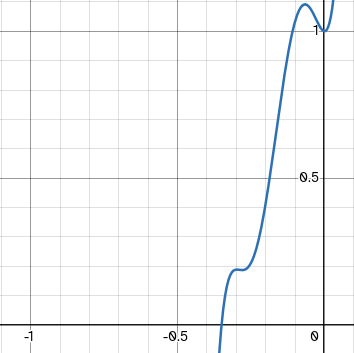
\includegraphics[width=0.45\textwidth]{assets/poly-negGrad.png}
  }
  \subfloat[Positive Gradient Speed Polynomial] {
    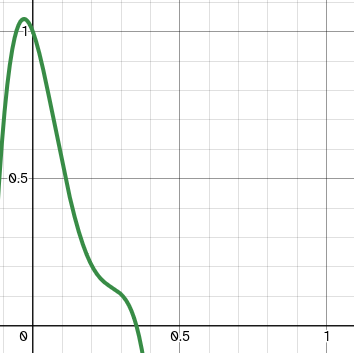
\includegraphics[width=0.45\textwidth]{assets/poly-posGrad.png}
  }
  \caption{Visual representation of the polynomials used in the \texttt{GradientSpeedFeature} to convert an input gradient $x$ to speed multiplier $y$.}
  \label{fig:gradspeed}
\end{figure}

To reduce computational complexity of solving these polynomials, the polynomial is split into two models: one for positive gradients, and another for negative gradients, with polynomial degree 5 and 6 respectively (see. \autoref{fig:gradspeed}). This approach reduces the number of multiplications required to solve, adding just a single sign check for the input gradient to direct solving to the correct model. The polynomials are customizable through the setting of the \texttt{positive\_coefficients}, and \texttt{negative\_coefficients} vectors.

The gradient of a terrain is constrained at all points to a range of -1 and 1, representing a range of 90 to -90. This is the case because gradients beyond these limits imply a reversal in direction, bringing the gradient back to within this range. Therefore, the polynomial outputs beyond these $x$ ranges do not need to be accurate. Both positive and negative gradients include maximum and minimum values where traversal is not possible. This is represented by the speed output returning a value $\leq{0}$, which is then snapped to 0, ensuring speeds remains non-negative.

\subsection{Logic Features}

Logic features are (usually) simple mathematical features, which take the value from one feature, or change the control flow of the cost function dependent on dependency output. These features likely do not require initialization or tagging logic, except potentially for caching results (the example implementations use the default blank logic).

\subsubsection{Inverse Feature}

The inverse feature is a simple feature used for division and as a basic relational feature for non-traversable features to be converted to a 0/1 speed multiplier.

Inverse features are defined using two template parameters, defining the input and output type. Each supported combination is defined independently which impacts the invert behaviour depending on the desired output.

Boolean to boolean inverting is simple, and implemented using \texttt{!} boolean inverting of the dependency value.

\begin{figure}[H]
  \centering
  \begin{lstlisting}
	template <>
	inline double InverseFeature<double, double>::Calculate(TsrState &state) {

		auto feature =
				std::dynamic_pointer_cast<Feature<double>>(this->dependencies[VALUE]);

		double value = feature->Calculate(state);

		if (value == 0) {
			return std::numeric_limits<double>::infinity();
		}

		return 1 / value;
	}
	\end{lstlisting}
  \caption{The implementation of the \texttt{InverseFeature} with \texttt{<bool,bool>} as input and output template parameters.}
  \label{lst:invert:doubledouble}
\end{figure}

For double to double inversion, the desire is to enable division, modelling $\frac{1}{x}$. To prevent division by zero, a check for $x = 0$ is done beforehand. This behaviour is undefined in mathematics, but the decision to return infinity was decided, because as $x \rightarrow{} 0$, the value $\frac{1}{x} \rightarrow{} \text{infinity}$. The implementation can be seen in \autoref{lst:invert:doubledouble}.

\subsubsection{Multiplier Feature}

The \texttt{add\_dependency} method is changed for this feature, to specify the input type of the dependency. Features by default must know in advance the input types, but this feature supports dynamic types through specifying the \texttt{DEPENDENCY\_TYPE}. Currently, \texttt{double}, \texttt{int}, and \texttt{bool} values are supported --- this is likely sufficient to model most features, as it allows floating point, integer, and snapping with boolean values.

The \texttt{Calculate} implementation fetches the values from each dependency. A default output of 1 is used if there are no dependencies, which enables this value to be multiplied by the values directly without affecting the correctness of the output (as $x \times{1} = x$). The output is modelled as a double, requiring casting \texttt{int} values before multiplication. For boolean values, \texttt{true} values multiply the output by 1, and \texttt{false} multiplies by 0. This boolean multiplication enables the inverse of existence for untraversable features to be directly multiplied with the speed multiplier feature, reducing the overall feature complexity and thus improving performance. Any multiplication by 0 results in an early output of 0, as any further multiplications follow the rule $0 \times{x} = 0$. This reduces the number of computations if 0 values are set as early dependencies.

\subsubsection{Conditional Feature}

Conditional features enable change in control flow, and are used by the default preset to override (i.e. not check for) water and terrain factors where paths exist.

\begin{figure}[H]
  \centering
  \begin{lstlisting}
	template <typename DataType>
	class ConditionalFeature : public Feature<DataType> {
	private:
		enum DEPENDENCIES { CONDITIONAL, A, B };

	public:
		using Feature<DataType>::Feature;

		DataType Calculate(TsrState &state) override {

			auto conditionalFeature = std::dynamic_pointer_cast<Feature<bool>>(
					this->dependencies[CONDITIONAL]);

			if (conditionalFeature->Calculate(state)) {
				auto feature =
						std::dynamic_pointer_cast<Feature<double>>(this->dependencies[A]);
				return feature->Calculate(state);
			} else {
				auto feature =
						std::dynamic_pointer_cast<Feature<double>>(this->dependencies[B]);
				return feature->Calculate(state);
			}
		}
	};
	\end{lstlisting}
  \caption{\texttt{ConditionalFeature} implementation, showing the dependency order is named through the \texttt{DEPENDENCIES} enum, and values only calculated when required.}
  \label{fig:conditional}
\end{figure}

To support any data type to enable further developers to create their own presets, the conditional feature is constructed so that the first dependency added must have a boolean output type. This is used as the conditional, and then two other dependencies are required, both matching the output type specified with the \texttt{DataType} template parameter (see. \autoref{fig:conditional}). The values of the output are only requested once the conditional value is known, improving performance, as both branches are never both evaluated.

\subsection{Coordinate System Conversion}

Warping raster datasets requires a different approach than warping vector datasets. For raster data, GDAL's \texttt{GDALWarp} tool was used, which handles resampling and re-projection of datasets. For vector datasets, \texttt{GDALTranslate} was used to warp the vector points and geometries. These tools ensure efficient and accurate coordinate system conversions.

The decision to use GDAL instead of developing custom warping tools was driven by GDAL's proven optimization for performance and memory management. These factors are critical for the efficiency of the routing algorithm, as computational overhead can significantly impact results. GDAL's C++ APIs are well-documented and support a wide range of input file types and projections, streamlining the implementation process.

\subsection{Uniform Cost Search}

\begin{figure}[H]
  \centering
  \begin{lstlisting}[language=c++]
	// Step 1. Check exit conditions
	while (!this->state.routes.contains(this->state.end_vertex)) {

		// Step 2. Select next node
		RouteNode current_node = cost_queue.top();
		cost_queue.pop();
		
		// Check if the best route is untraversable
		if (current_node.gCost == std::numeric_limits<double>::infinity()) {
			// ...
			throw std::runtime_error("Could not find safe path");
		}

		// Record the best-known route to this vertex
		this->state.routes[current_node.vertex] = current_node;
		this->state.current_vertex = current_node.vertex;

		// Step 3. Calculate neighbour cost
		// ...
	}
	\end{lstlisting}
  \caption{The main uniform cost search algorithm implementation.}
  \label{fig:impl:search:mainloop}
\end{figure}

The \texttt{Router} class gives the implementation of the uniform cost search algorithm. Because the search graph is a continuous 3D surface mesh, the nearest vertex in the TIN must be found before search begins. \texttt{CalculateNearestVertexToPoint} uses CGAL's \texttt{locate(point)} available for Delaunay triangulations, which finds the faces at the given positions. If the points given are outside the mesh boundary, then the function returns a \texttt{nullptr}, and an error can be thrown as the search domain does not include the start or end point.

\autoref{fig:impl:search:mainloop} shows the main search loop. The priority queue is initialized using a \texttt{std::priority\_queue<RouteNode>}, this holds the routes explored to nodes not yet searched. The \texttt{RouteNode} class contains a pointer to the vertex, and it's parent for reconstruction, as well as the cumulative cost \texttt{gCost}, and a pointer to the face that is being traversed over when following the edge.

A custom \texttt{CompareNode} ensures that the priority queue gives the smallest \texttt{gCost} during node selection --- maintaining the best-first approach.

The minimum costs are represented through the storage of their associated \texttt{RouteNodes} in a \texttt{std::unordered\_map}, linking vertex pointers to \texttt{RouteNodes}. Unordered maps offer $\mathcal{O} (1)$ time complexity to store and fetch values. This is vital for performance, as values are fetched many times in one search loop to check if nodes have already been searched. Additionally, the worst-case size of this map is the number of vertices in the mesh.

When routing an infinite cost (defined using \texttt{std::numeric\_limits}) represents that a route is untraversable. If when routing the next node selected has this infinite cost, then it means that the cost to the target will be at minimum infinite, as costs are cumulative and non-negative. Therefore, the routing algorithm tells us when no safe route exists. Untraversable routes are defined by the cost function, and can be configured to represent any completely undesirable route features.

\begin{figure}[H]
  \centering
  \begin{lstlisting}[language=c++]
	// Get the faces connected to the vertex
	auto faceCirculator = current_node.vertex->incident_faces();

	// Validate there is at least 1 connected face
	if (faceCirculator != nullptr) {
		auto faceCirculatorEnd = faceCirculator;
		do {
			auto face = faceCirculator;
			if (dtm.is_infinite(face)) {
				continue;
			}

			// Search each vertex in each face
			for (int i = 0; i < 3; i++) {
				Vertex_handle connectedVertex = face->vertex(i);

				// Skip if it is the same vertex or already visited or out-of-bounds
				if (connectedVertex == current_node.vertex) { continue; }
				if (this->state.routes.contains(connectedVertex)) { continue; }
				if (!boundary.IsBoundedSafe(connectedVertex->point())) { continue; }

				// Calculate cost
				RouteNode node(connectedVertex, face);
				this->state.next_vertex = connectedVertex;
				node.gCost = current_node.gCost + CalculateTrivialCost(fm, this->state);
				node.parent = current_node.vertex;

				cost_queue.push(node);
			}
		} while (++faceCirculator != faceCirculatorEnd);
	}
\end{lstlisting}
  \caption{The process of searching neighbouring search node edges using the TIN mesh representation.}
  \label{fig:impl:search:edges}
\end{figure}

After selecting the next node, the costs of traversing over edges to connected nodes is done. Each edge in the TIN mesh corresponds to one or two search edges, as we associate a particular search with a face, and edges in the TIN are connected to a maximum of two faces. This enables following data contours along either side using the same edge such as following alongside the edge of a river.

The process of selecting and calculating costs of adjacent nodes is give in \autoref{fig:impl:search:edges}. Initially, due to each node requiring up to two searches per face, testing was done by fetching the connected edges, and then the two connected faces of those edges if the target node was not already searched. However, due to the \texttt{incident\_edges} and \texttt{incident\_faces} having to traverse the mesh in CGAL, a faster approach is to fetch the incident faces to the current vertex, and then validate each vertex connected. This requires repeated checks for the same nodes, but only requires one mesh traversal \texttt{incident\_faces}, as vertices can be fetched directly using \texttt{face\_handle.vertex(i)} where \texttt{i} is the vertex index (1,2 or 3).

\section{Results and Analysis}

This section explores how different configurations and inputs affect the performance of the router in terms of both performance and quality of routes. Visualization of the generated meshes themselves is done through exporting the mesh to an object file, which is imported into the popular 3D modelling tool blender.

\subsection{Final Configuration Mesh Generation}

Objectively determining the quality of the mesh triangulation is not possible, as there are an infinite number of triangulations that could represent the same terrain. However, we can identify features in meshes which may give insights into their quality.

\begin{figure}[H]
  \centering
  \subfloat[TSR's Solid Mesh] {
    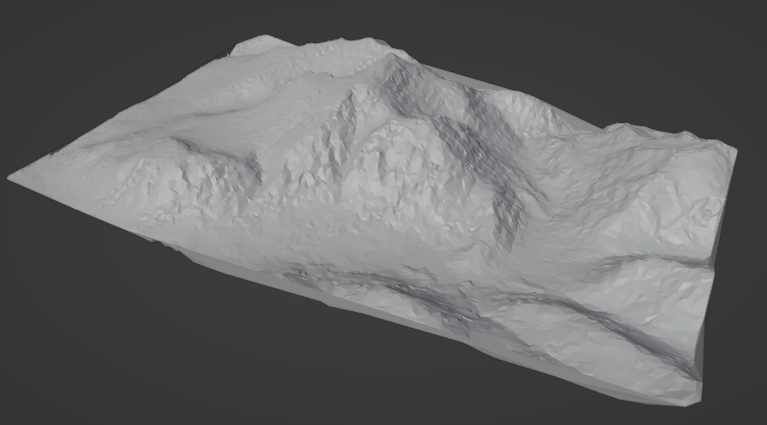
\includegraphics[width=0.4\textwidth]{assets/benNevis-perspective-solid.png}
  }
  \subfloat[Google Earth's Topography] {
    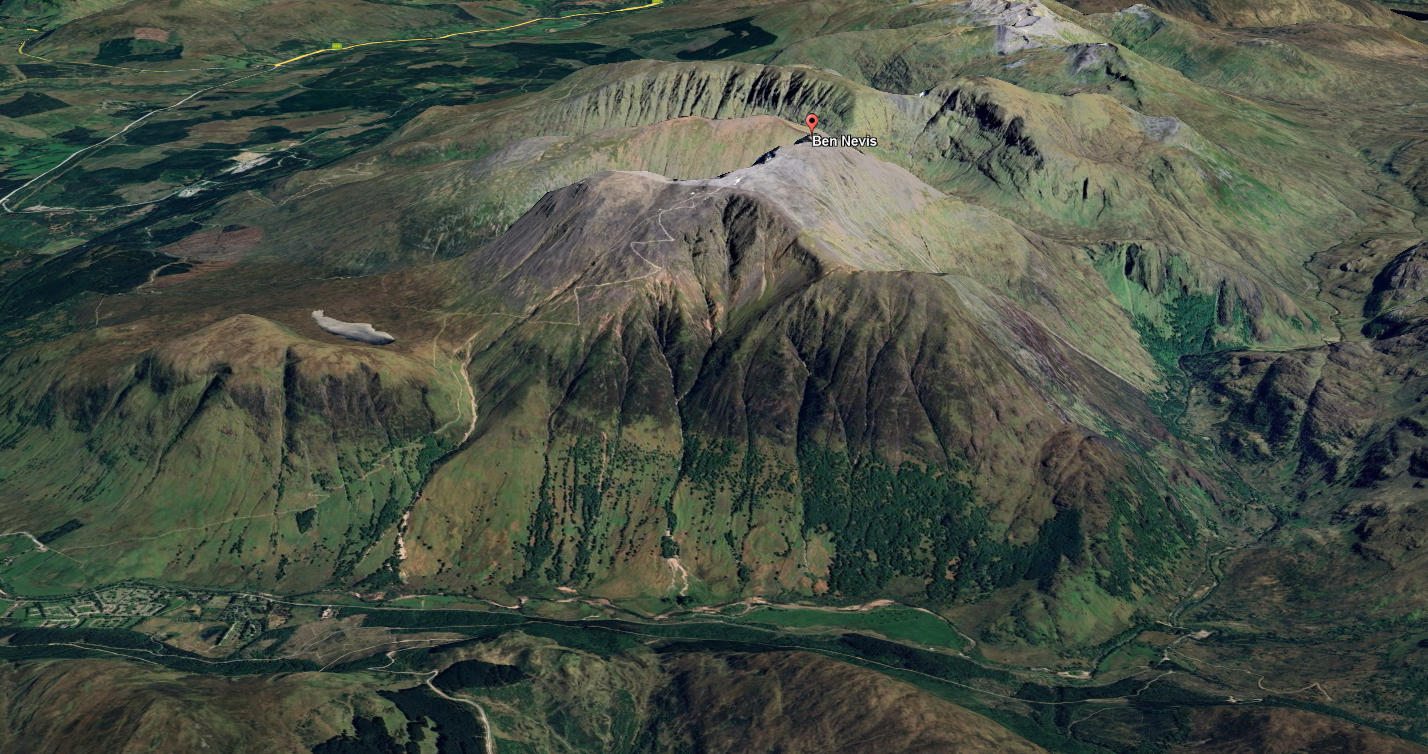
\includegraphics[width=0.4\textwidth]{assets/benNevis-gearth.png}
  }
  \caption{Visual comparison of meshes of Ben Nevis. The generated mesh from this application on the left, and Google Earth's topology mesh on the right.}\label{fig:mesh:benNevis:comparison}
\end{figure}

We initially evaluate the accuracy of the generated TIN mesh by visually comparing it to Google Earth's topography, as shown in \autoref{fig:mesh:benNevis:comparison}. Google Earth's horizontal accuracy (30 m) and height accuracy (10 m), are only marginally higher than the COP-30 DEM used in this project. Therefore, significant differences between the two meshes are likely a result of the mesh simplification process.

However, one limitation of this comparison arises from the differing projections used. Google Earth uses the WGS84 projection scheme, not UTM, and so there are some scaling and warping due to this difference. However, general features should still be identifiable.

As seen in \autoref{fig:mesh:benNevis:comparison}, the primary topographic features in the Google Earth mesh are all visible in the generated mesh. Nonetheless, improvements could be made in finer details such as sharp angles in mountain ridges, and sudden valleys.

In addition, the DEM data used fails to accurately model the topography of areas underwater, as seen in the bottom left of \autoref{fig:mesh:benNevis:comparison}. However, this does not impact the quality of most routes as usually water is completely avoided, or otherwise route following the route an individual would swim at the surface of the water.

\subsubsection{Edge Detection}

\begin{figure}[H]
  \centering
  \subfloat{
    \centering
    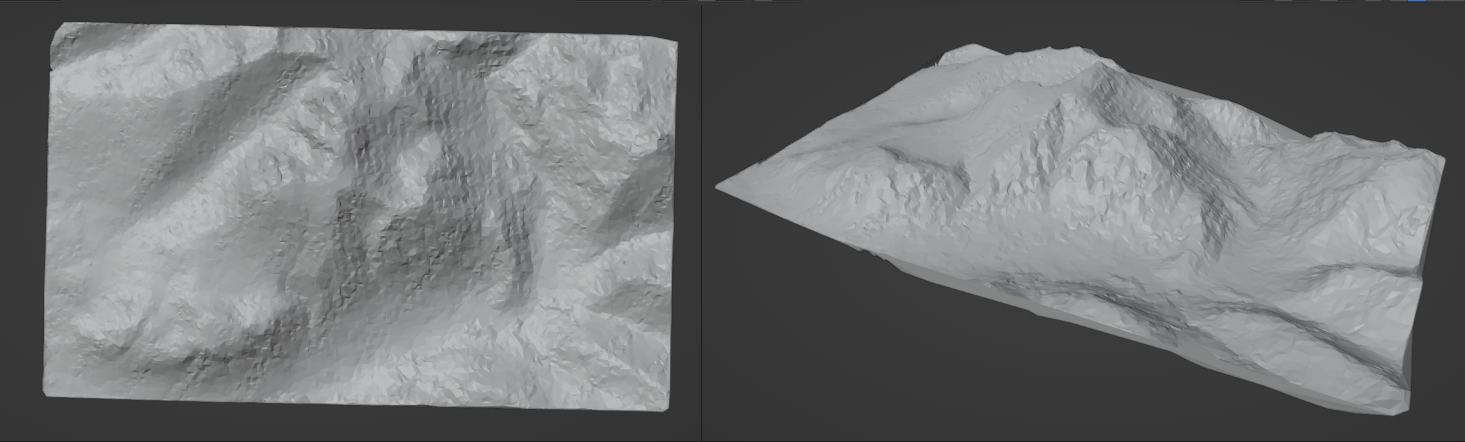
\includegraphics[width=0.8\textwidth]{assets/benNevis.png}\label{fig:mesh:benNevis:solid}
  }\\
  \subfloat{
    \centering
    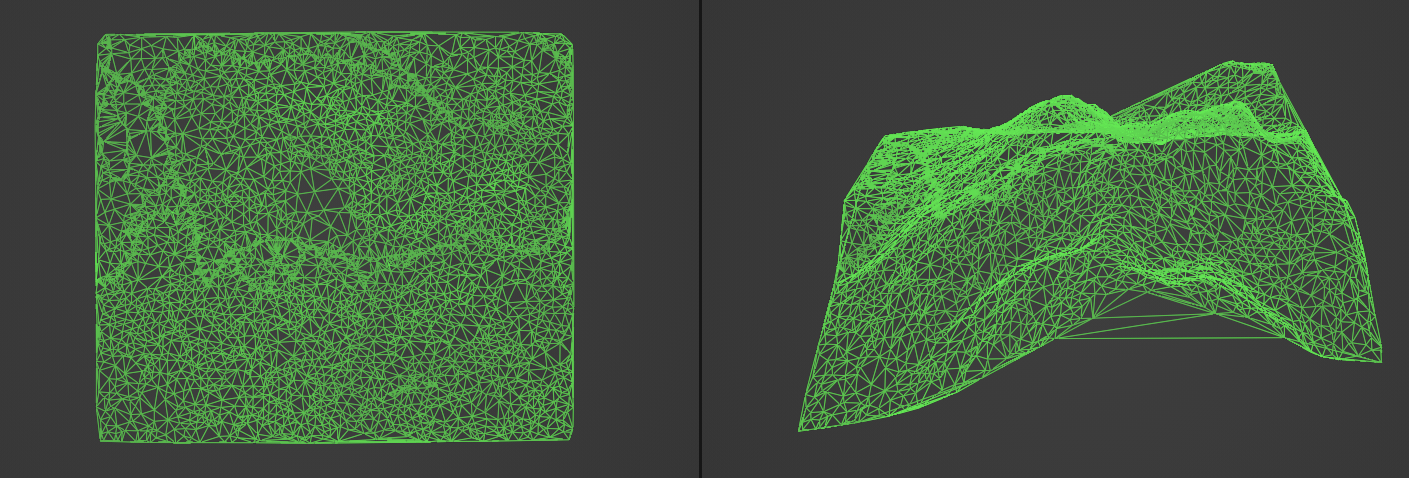
\includegraphics[width=0.8\textwidth]{assets/benNevis-wire.png}\label{fig:mesh:benNevis:wireframe}
  }
  \caption{Final model of Ben Nevis, with path, water-feature, and terrain-type contours applied. A solid and wireframe render are shown, in both top-down orthographic, and side-on perspective views. Demonstrating a recognizable, but noisy and non-perfectly optimized mesh.}\label{fig:mesh:benNevis}
\end{figure}

\autoref{fig:mesh:benNevis} demonstrates the quality of the mesh produced with the default preset. The top-down orthographic view shows the water and paths with higher resolution than the DEM mesh, whilst the solid views show how these features do not impact the topography of the mesh.

\subsection{Generated Routes}

This section analyses the routes generated by this route planner, considering differences between different cost function pre-sets. Evaluation therefore will be focused on the success to which the cost function generates routes according to the goal of the model.

The first preset can be found in \autoref{fig:cost:example:1} and models estimated traversal time.

\subsection{Path Feature}

A significant draw back to the current implementation derives from the use of CGAL's insert constraint function. When constraints intersect, they must be split at the intersection point to maintain the validity of the mesh. This works well for most features, but where keeping track of constrained edges, such as which edges are paths, the automatic subdivision breaks this.

Solutions to this issue could be implemented. First, developing a custom mesh representation, and implementing a custom constraint addition function could allow paths to be directly tagged.

Alternatively, CGAL enables defining a custom \texttt{Vertex\_base} class which can be used to override the default constructor for vertices, adding custom attributes to each vertex. When inserting into the mesh using \texttt{tin.insert}, the vertex handle is returned, allowing a standard vertex tag to be applied. When inserting constraints, we can loop over vertices in the graph, and check for vertices who have the default, unset tag value. This will give the set of vertices creating that constraint.

\subsection{Quantitative Analysis}


The route planner has multiple major factors influencing the performance of any particular execution which will be discussed and analysed here. Testing was completed on the same machine (specs are given in \autoref{appendix:specs}).

\subsubsection{Mesh Size}

\begin{figure}[H]
  \centering
  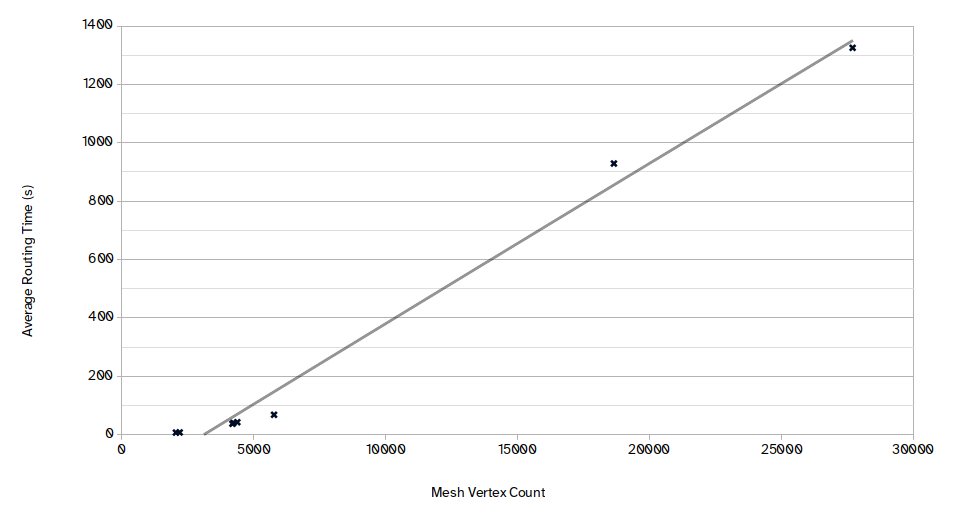
\includegraphics[width=\textwidth]{assets/searchtime-vertices.png}
  \caption{The impact of the mesh size (vertex count) on the search time after setup.}
  \label{fig:eval:vertices}
\end{figure}

From testing, the search algorithm appears to have a linear time-complexity with regard to the number of search graph nodes (see. \autoref{fig:eval:vertices}). This suggests that optimizations and multi-threading may be useful in improving the scale of searches feasible, as the underlying algorithm will not exponentially take longer. This is a great success for the search algorithm and preset created, however, this is not guaranteed depending on the cost function constructed.

\subsubsection{Caching}

\begin{figure}[H]
  \centering
  \subfloat[Logarithmic Scale]{
    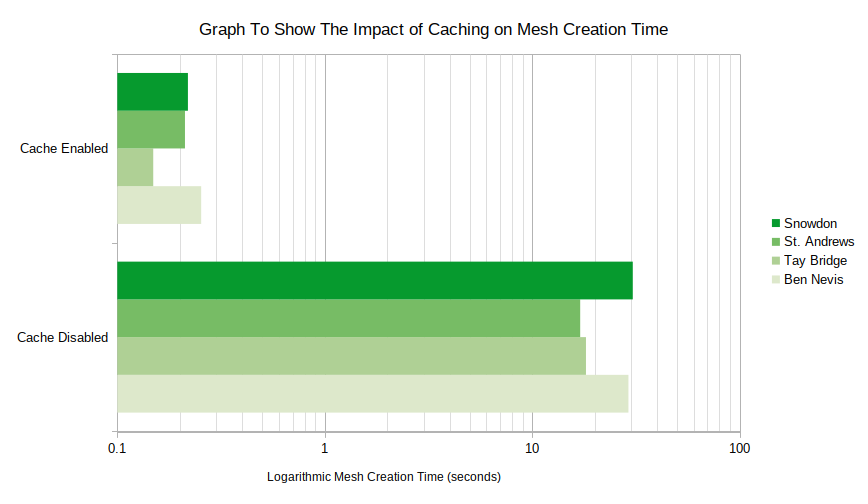
\includegraphics[width=0.45\textwidth]{assets/eval-cache-log.png} % chktex 35
  }
  \subfloat[Linear Scale] {
    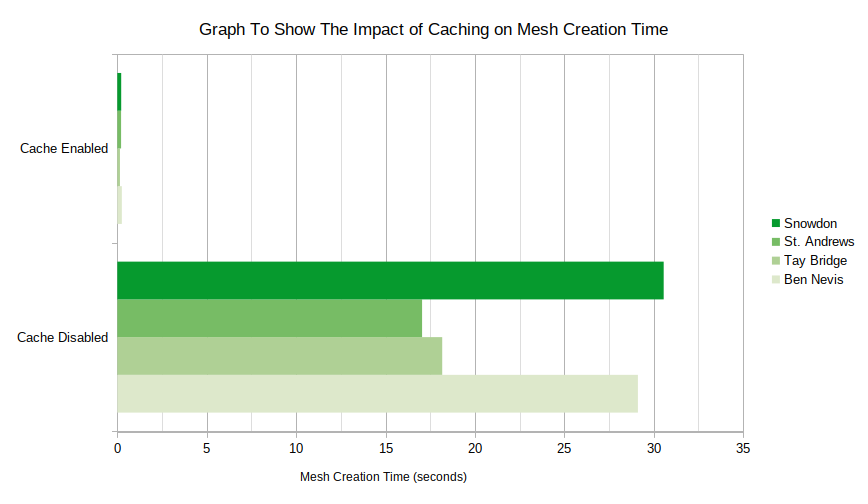
\includegraphics[width=0.45\textwidth]{assets/eval-cache.png}
  }
  \caption{Caching has a dramatic impact on the initial mesh construction.}
  \label{fig:eval:cache}
\end{figure}

The impact of caching was evaluated by routing through the same points two times. \autoref{fig:eval:cache} shows the impact on the mesh construction time is dramatic, as all tiles are cached, meaning no API calls are required. These performance increases will be essential in creating a user-friendly application for a general audience.

\subsection{Qualitative Analysis}

This section gives examples of routes generated by preset configurations, to show their impact on routing decisions.

\subsubsection{Gradient}

\begin{figure}[H]
  \centering
  \subfloat[Routing up-hill not considering gradient] {
    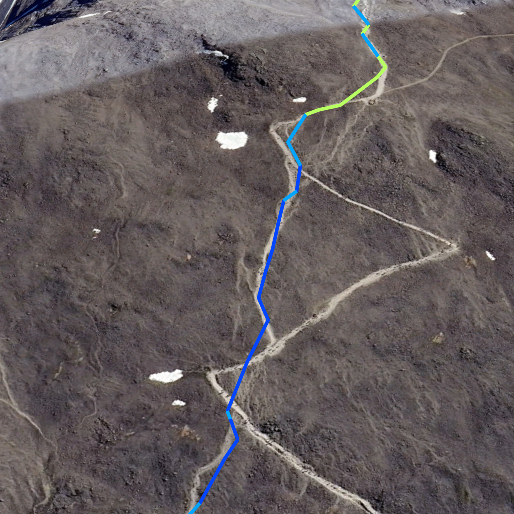
\includegraphics[width=0.45\textwidth]{assets/benNevis-up-noGrad.png}
  }
  \subfloat[Routing up-hill considering gradient] {
    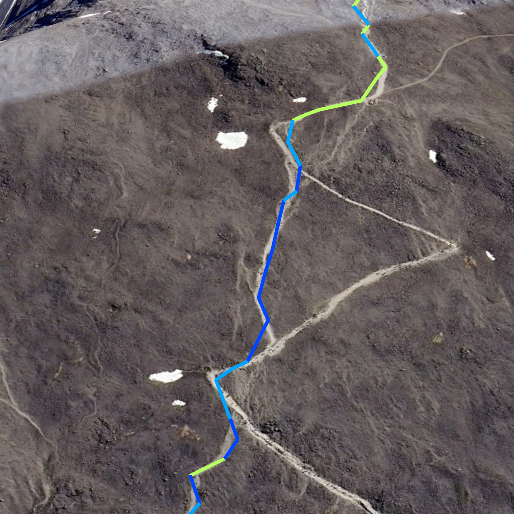
\includegraphics[width=0.45\textwidth]{assets/benNevis-up.png}
  }
  \\
  \subfloat[Routing down-hill not considering gradient] {
    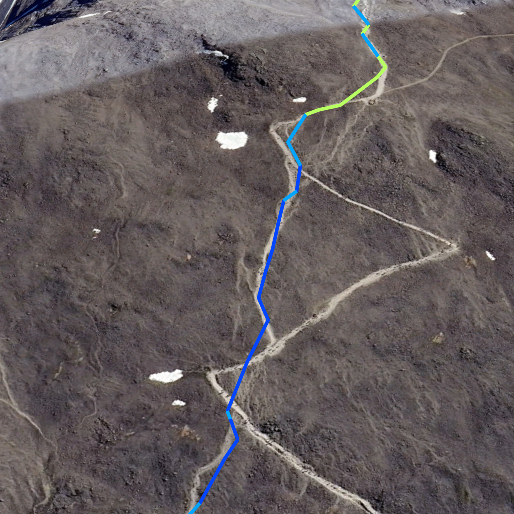
\includegraphics[width=0.45\textwidth]{assets/benNevis-down-noGrad.png}
  }
  \subfloat[Routing down-hill considering gradient] {
    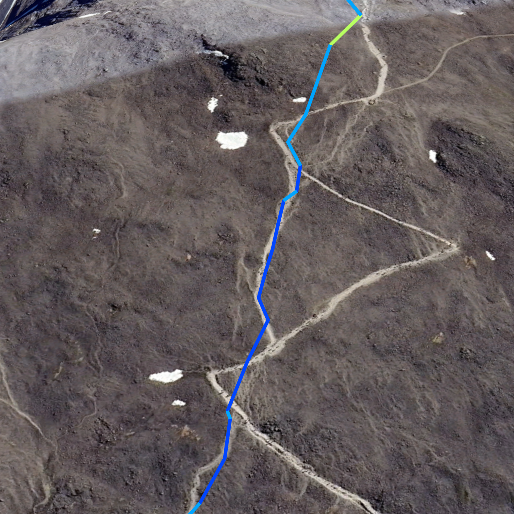
\includegraphics[width=0.45\textwidth]{assets/benNevis-down.png}
  }
  \caption{Demonstration of the impact of the gradient and gradient-speed features on routing decisions, considering positive and negative gradients differently.}
  \label{fig:benNevis:gradient}
\end{figure}

\autoref{fig:benNevis:gradient} gives a comparison between the differences between routing between the same points up-hill and down-hill, comparing the default preset considering gradient to the same preset with gradient consideration removed.

As expected, when gradient is not considered, the upwards and downwards routes generated are identical. \autoref{fig:benNevis:gradient} suggests the router successfully models the different impact of positive and negative gradients, due to the zigzag pattern being visible where gradient is considered. In addition, the upwards direction shows emphasized zigzagging compared to the downwards direction when considering gradient --- demonstrating the difference in speed influence evaluation for positive and negative gradients.

The optimal walking pattern when traversing a steep positive and negative gradient is a zigzagging pattern \autocite{horiuchi2015comparisons}. Humans are impacted differently for positive and negative gradients. For example, walking slightly up hill will have a lightly negative impact on walking speed. Walking slightly downhill has a lightly positive impact on walking speed. As negative and positive gradients increase, the walking speed is increasingly then negatively impacted, but at different rates for each direction, eventually both having a point where humans cannot traverse by walking.

\subsubsection{Water}

\begin{figure}[H]
  \centering
  \subfloat[Image of the terrain around the Cameron reservoir, Fife with the desired start and end points shown.] {
    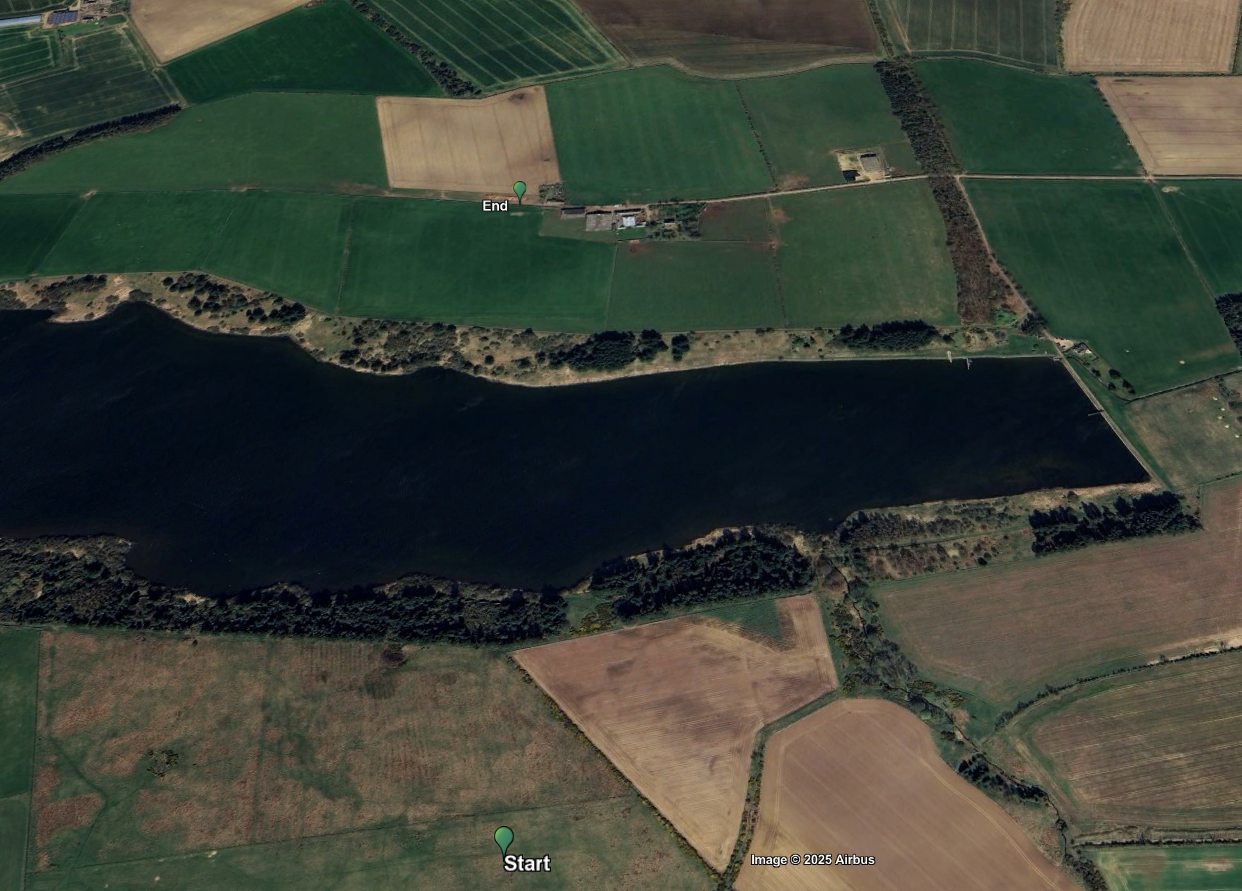
\includegraphics[width=0.45\textwidth]{assets/reservoir-blank.png}
  }
  \subfloat[The suggested route generated with the default preset.] {
    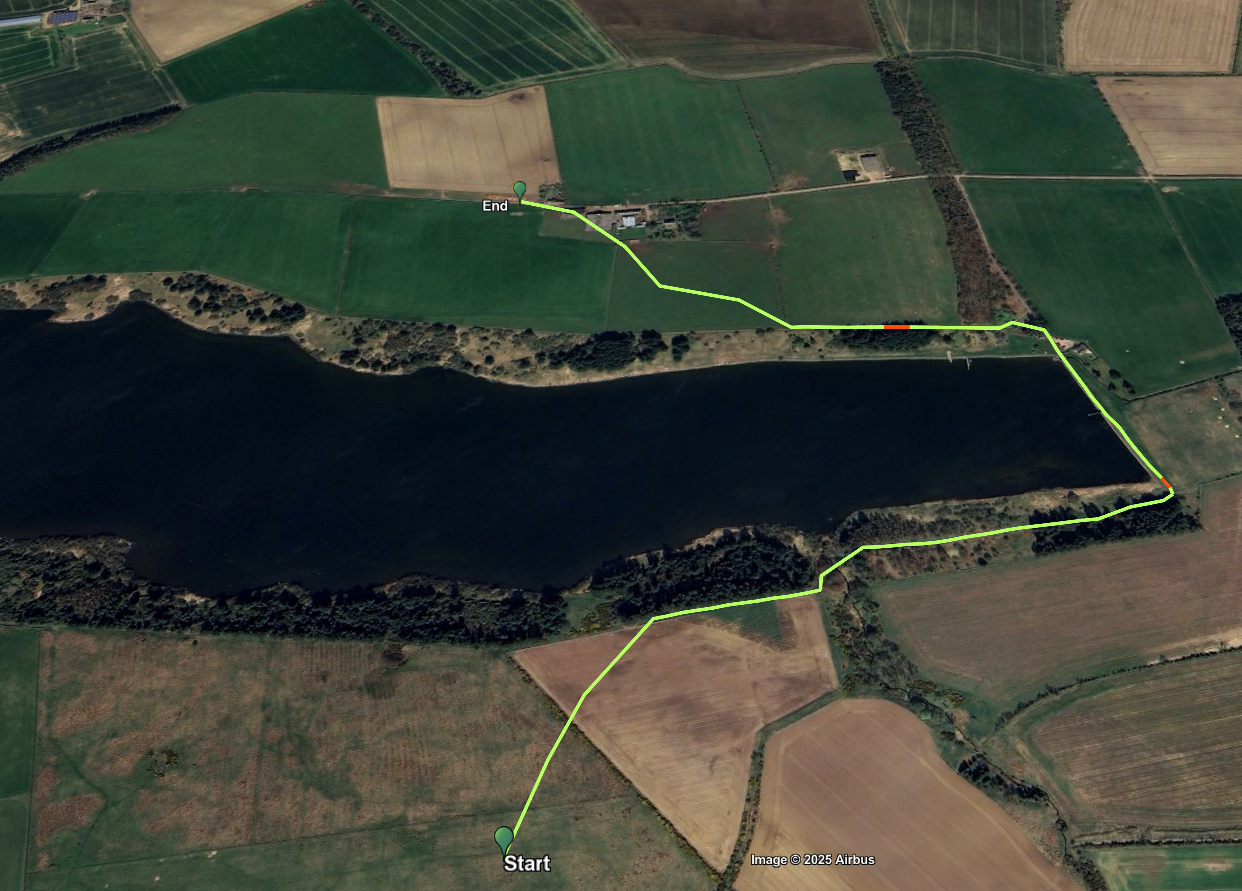
\includegraphics[width=0.45\textwidth]{assets/reservoir-route.png}
  }
  \caption{Demonstration of the router avoiding water closely along its edge.}
  \label{fig:reservoir}
\end{figure}

The water feature is used in the default preset to completely avoid areas of water. \autoref{fig:reservoir} shows the accuracy of the constraint approach to tagging features, accurately avoiding closely along the edge of the water, following along a footpath.

\begin{figure}[H]
  \centering
  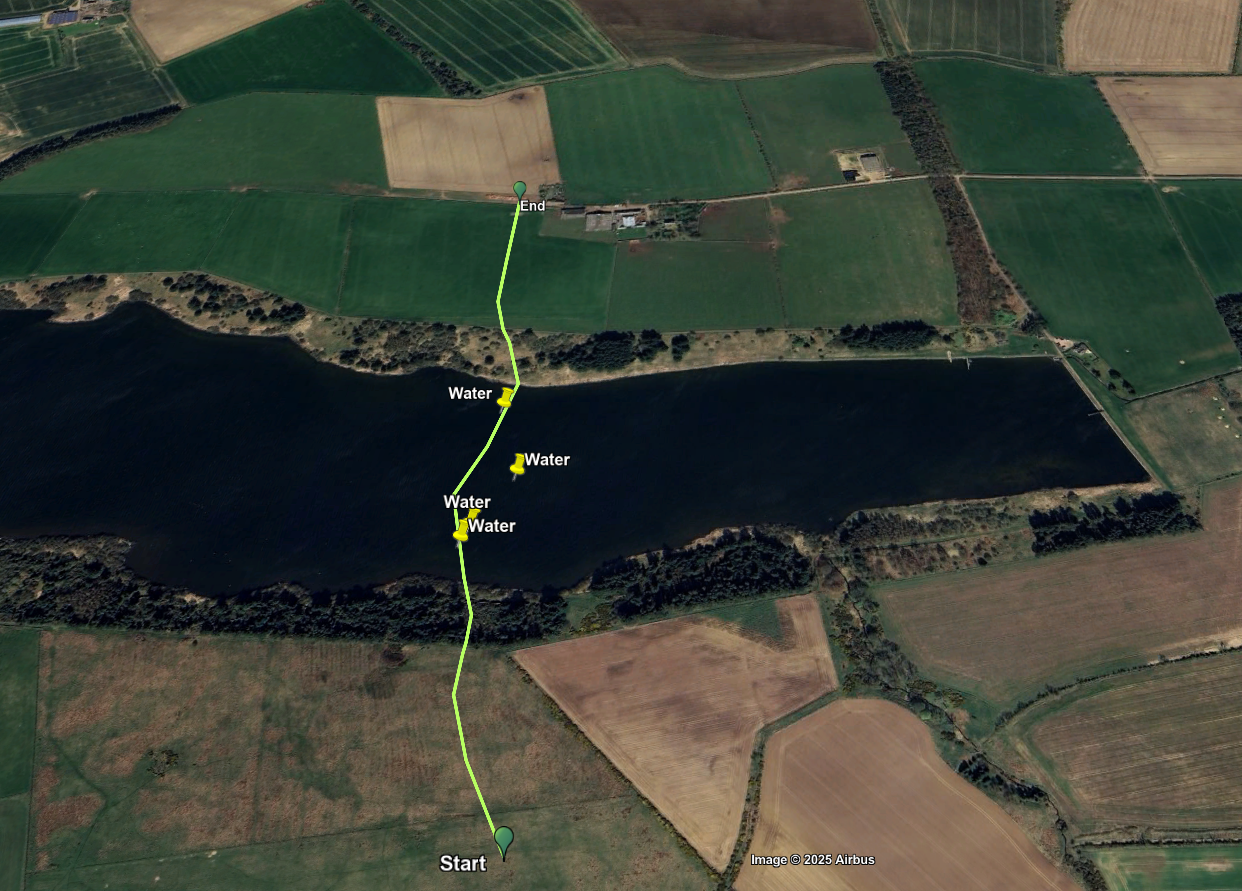
\includegraphics[width=0.45\textwidth]{assets/reservoir-swim.png}
  \caption{Demonstration of how changing the preset to enable swimming impacts the generated route.}
  \label{fig:reservoir:swim}
\end{figure}

We can then see how water impacts the route through the swimming preset in \autoref{fig:reservoir:swim}, which is identical except swimming is enabled which reduces speed to 89\% compared to walking, instead of completely blocking swimming.

\section{Evaluation and Critical Appraisal}

The results and analysis in the previous section enable an evaluation to be done on the project in reference to the aims and objectives set out in the initial aims and objectives requirements specification. This section will go through each requirement, and discuss the level to which the submission meets each of the given requirements.

\subsection{Aims}

The primary aim for this project was to contribute to the development of tools to make walking and running more accessible to those lacking safe roads, or to those who prefer not being restricted to roads and paths. The routing framework is successful in enabling users to define their own preferences in terms of the features through the configuration of features, and the cost function as a whole.

\subsection{Objectives}

\subsubsection{Primary Objectives}

The primary objectives are the primary measure of the success of the project. Here, each will be referenced and discussed.

\begin{itemize}
  \item Modular Routing Algorithm

        This objective was met. The cost function based on defining a DAG consisting in features enables any logic to be constructed within its structure. Further developments to improve performance would have been beneficial, but the result is a good proof of concept.

  \item Route Visualization

        The Google Earth routes generated, with markers specifying warnings for potentially hazardous areas around the route successfully visualize the output, and gives users a change to evaluate the route and potential safety considerations.

  \item Critical Evaluation of Presets

        A fair amount of analysis was done on the route planner and outlined in this document. However, further analysis would be beneficial in terms of a full performance breakdown of specific areas of computation to guide future optimizations. The qualitative analysis gives good insight into proving the cost functions is modelling factors successfully.

\end{itemize}

\subsubsection{Secondary Objectives}

\begin{itemize}
  \item Additional Cost Function Presets

        This was successfully implemented, demonstrating the versatility of the routing algorithm and cost function framework. Further development of real-world cost function presets would have been useful in further demonstrating the accessibility of the router.

  \item Additional Cost Function Features

        The addition data features were not implemented due to time limitations, however, logic features were implemented, enabling complex relationships such as if-then-else statements to be made. These logic statements help reason about the cost function model.

\end{itemize}

\subsection{Tertiary Objectives}

\begin{itemize}
  \item Interactive User Interface

        This was not implemented due to time limitations, and a prioritization of the cost function itself. However, some design ideas were considered and outlined in \autoref{section:improvements:ui}.

  \item Route Generation Animation

        This was also not implemented. This would have added insight into the routing decisions. However, the warnings KML output serves a similar purpose, as it shows warnings for searched areas, and so it may be useful in showing where the router came to barriers.

\end{itemize}

\section{Potential Improvements \& Future Projects}

This project aimed at forwarding research into accessible off-road route planning. Due to the scale of route planning off-road, and the limited previous research, this solution to the problem is not perfect. This section discusses these potential improvements in detail in addition to those discussed in the evaluation section. In addition, a discussion discussed research that would be required in other fields to solve some limitations of this project.

\subsection{Interactive Cost Function UI}\label{section:improvements:ui}

\begin{figure}[H]
  \centering
  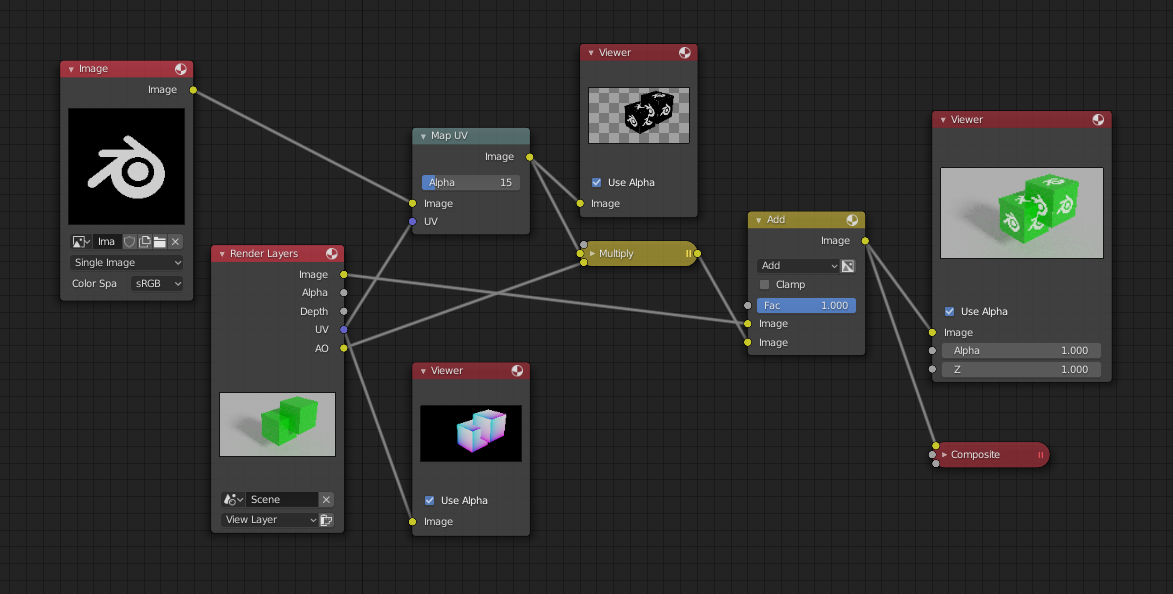
\includegraphics[width=\textwidth]{assets/blender-compositor.png}
  \caption{Blender's compositor interface, allowing interactive customization of the rendering pipeline. Image taken from Blender's user manual \autocite{blenderCompositor}.}
  \label{fig:blender-compositor}
\end{figure}

A user interface enabling users to drag and drop features onto a user interface, and control the configuration options interactively would be a huge development towards this tool being useful for a general audience. \autoref{fig:blender-compositor} shows Blender's compositor tool, allowing users to define their own DAG for how an object and scene gets rendered. This same interface could be applied to this routing algorithm, which features as nodes, connected defining dependency relationships, and options within the nodes relating to the configuration options. This interface could output either code to be used in preset setup, or it could output JSON, which could be parsed by a \texttt{FeatureManager} and setup.


\subsection{Tag Chunking}

Currently, the water and terrain type features tag the entire mesh faces when setting up. This is to avoid constant IO operations with opening the file for each face searched. However, a middle ground approach may allow faces to be fetched when required. For example, when the Calculate function is called, the face required could be fetched, along with a certain range of adjacent faces. It is my hypothesis that often than not, searches stay following routes around a low-cost area for some time, and so caching these local values would reduce IO operations. The current setup imposes a resource limit on the number of faces in the graph, as every face must be cached in memory. This could enable lower simplification values to be used.

\subsection{Parallelized Feature Setup}

Where this implementation parallelizes mesh construction, the setup of individual features could be parallelized. However, this would require careful consideration as it may be desirable to allow features to interact in the setup phase, to allow for caching of calculated values using dependencies. A very basic parallelization that would not require these considerations would be of the API calling and chunking of data features, as with the TIN construction from DEM data.

\subsubsection{Cost Function Caching}

Whilst there is pre-caching of many data-values, additional caching at-runtime for a particular cost-function evaluation may dramatically improve performance for more complex models. The DAG structure enables multiple nodes to add dependencies to the same node as long as there are no cycles. However, each of these nodes calls the Calculate function separately. One solution to this problem may be to cache values when a method is called first, and so subsequent calls do not require redundant calculation.

\subsection{Iterative Cost Function}

Due to new stack frames being generated at each function call, the current recursive design of the cost function limits its maximum size and complexity, as each dependency runs whilst the parents function is still in scope, thus using memory. Performance in all aspects could be improved through the conversion of this recursive design to an iterative approach.

This may involve using the \texttt{FeatureManager} to handle all calculate requests. Instead of features directly calling calculate to their dependencies and casting these results, the feature manager could maintain a list of the dependencies, and iteratively follow the DAG, not calling calculate until a leaf-node is found (one with no dependencies). The leaf nodes could then be calculated, and their values passed as input when calling calculate on its dependent.

However, challenges arise in maintaining the ability for features to output any type, as the feature manager would have to be able to handle the arbitrary output type, and input it into features.

\subsection{Improvements to Features}

\subsubsection{Distance Dependent Features}

The implementation of the water feature created allows avoiding or heavily punishing swimming. However, it may be helpful to set a maximum swimming distance, to ensure routes through overly large areas of water are suggested.

This could be done by first getting the distance for the current edge if it is over water. If beyond a determined maximum swimming length, then it could return an infinite cost (implying non-traversable). If lower, then the source vertex's parent could be fetched from the \texttt{bestRoutes} map in the state. We can repeatedly check if that edge is over water, and add the distance to a running total until you reach land, to get the total current water distance.

A potential alternative approach would modify the \texttt{RouteNode} class to cache results where needed seeing similar performance benefits.

\subsubsection{Improve Contour Extraction}

The current implementation allows relevant data features to specify the level of simplification is applied to the contours extracted from datasets. This is suitable for binary data such as water which either exists or not. However, for categorical data, all borders are simplified to the same extent. In the case of datasets such as terrain data, it may be helpful to be able to specify the level of simplification for each data value --- enabling stricter borders to be represented around hazardous terrain types such as bog.

\subsubsection{Representing Streams}

The current implementation fails to properly represent streams. The \texttt{WaterFeature} data from OpenStreetMap gives the geometry of most water features. However, very thin and sometimes large water features (such as streams) can be represented as vector lines with no geometry. This means the face-tagging approach used for water features does not accurately represent these water features.

A potential solution would be to seek alternative datasets specifically designed to represent water geometry. Alternatively, it may be possible to pre-process these water features, and thicken their line width. By enforcing a minimum line-size, we can ensure faces are created and tagged. However, this approach does not perfectly model the real-world, and so further options may be optimal.

\subsubsection{Path Identification}\label{section:improvements:paths}

A relatively simple but effective addition to the \texttt{PathFeature} would be to return the category of path/road. Currently, roads/paths are equally weighted. However, many users would prefer to traverse over paths, and sometimes explicitly would like to avoid main roads. The overpass API by default returns GeoJSON containing the geometry of the paths/roads, along with a large amount of additional data such as type, surface, and access restrictions --- each of these could be extracted during data processing and stored in a data structure along with the geometry.

\subsection{Removing UTM Zone Restrictions}\label{section:improvements:zones}

This submission does not support areas outside UTM zone 30. This covers most of the UK, but the goal of accessible off-road routing is not truly complete until everyone around the world has access to it. Aside from feature data covering these areas, which could relatively simply be implemented, the projection from and to UTM coordinates, and the alignment of different zones is a big challenge, but would greatly increase the potential utility of the application.

Converting a point from WGS84 / a global projection scheme can be done simply by checking which zone the latitude/longitude values fall in, and whether the coordinate is on the northern or Southern Hemisphere. Converting a point back to a different coordinate scheme requires knowing this information.

Additionally, projecting points to UTM results in relative coordinates from the origin for that zone. These coordinates could be fetched, and added as offset when constructing the final mesh from chunks in different zones. Additionally, care to split chunks at the borders of zones is required --- resulting in irregularly sized chunks around zone boundaries.

\section{Conclusion}

The success of this project hinges on its developments into the understanding of the possibilities and barriers to the creation of generalized off-road route planning. The resulting application has a broad capacity to accurately model both mathematical concepts, and physical/psychological research into the impact of terrain features such as terrain-type, gradient, and fear on route preference.

This project adds a great deal to the understanding of off-road route planning using geometric terrain representations; suggesting that further optimization and research into constructing quantified model of walking speed and preference would greatly benefit pedestrian access to safe walking routes. Higher resolution data, more advanced processing techniques, and configuration tuning would also all aid in this pursuit.

\pagebreak

\nocite{esa2024dem}
\nocite{cgal:eb-24b}
\nocite{gdal}
\nocite{wiki:osm}
\nocite{gtest}
\nocite{fmtlib}
\nocite{opencv_library}
\nocite{oneTBB}
\nocite{tin_terrain_logging}
\nocite{libboost}
\nocite{geographiclib}
\nocite{gearth}
\nocite{blender}

\printbibliography[heading=bibnumbered]{}

\pagebreak
\begin{appendices}

  \section{Testing PC Specification}\label{appendix:specs}

  \begin{itemize}
    \item \texttt{OS: AlmaLinux 9.5 x86\_64} % chktex 29
    \item \texttt{Kernel: Linux 5.14.0-503.19.1.el9\_5.x86\_64}
    \item \texttt{CPU: 11th Gen Intel(R) Core(TM) i5-11400 (12) @ 4.40 GHz}
    \item \texttt{GPU 1: NVIDIA NVS 310}
    \item \texttt{GPU 2: Intel UHD Graphics 730 @ 1.30 GHz [Integrated]}
    \item \texttt{Memory: 30.86 GiBs}
  \end{itemize}

  \section{System Requirements}

  The following is a list of required c++ libraries that need to be installed, including versions used in development:

  \begin{itemize}
    \item \texttt{GDAL} (v3.4.3) --- GIS data processing
    \item \texttt{CGAL} (v5.6.2) --- Delaunay triangulation and mesh processing
    \item \texttt{oneTBB} (v2.13) --- Parallelization
    \item \texttt{OpenCV} (4.10.0) --- Computer Vision
    \item \texttt{GeographicLib} (v26.1.0) --- Point projection conversion
    \item \texttt{simdjson} (v3.6.0) --- JSON parsing (automatically fetched by CMAKE)
    \item \texttt{Eigen} (v3.3) --- parallelization for CGAL
  \end{itemize}

  \section{Compilation Instructions}

  To build the library and router, first setup the build directory:

  \begin{lstlisting}[language=bash]
	$ cd tsr-cli
	$ mkdir build && cd build
\end{lstlisting}

  \noindent Then configure with \texttt{cmake}, making sure to set configuration option values as appropriate:

  \begin{lstlisting}[language=bash]
	$ cmake .. -G Ninja -DCMAKE_BUILD_TYPE= -DTSR_TEST=
\end{lstlisting}

  \vspace*{-2em}

  \begin{itemize}
    \item \texttt{TSR\_TEST=ON/OFF}

          Specify whether to build test suite.

    \item \texttt{CMAKE\_BUILD\_TYPE=Release/Debug}

          Specify build type. Release is far more performant, but Debug contains much more logging information.
  \end{itemize}


  \noindent The library, CLI app, and tests can then be compiled using one of the following:

  \begin{lstlisting}[language=bash]
	# Compile everything
	$ ninja

	# Compile just the library
	$ ninja tsr

	# Compile the tests
	$ ninja test-tsr

	# Compile the cli application
	$ ninja tsr-cli
\end{lstlisting}

  \pagebreak
  \section{User Manual}

  For the CLI application, refer to the user manual below:

  \begin{lstlisting}[]
	Usage: 
			tsr-cli [options] <start_lat> <start_lng> <end_lat> <end_lng>
				Route between the given start and end points
			tsr-cli [options] --example  
				Route between a set of example start and end points
			tsr-cli [options] --help
				Print this help message

		Options:
			--radii-multiplier  Radii multiplier to apply to domain size
	\end{lstlisting}

  \pagebreak
  
\includepdf[pages=1, scale=0.8, pagecommand=\section{Ethics Self-Assessment Form}\label{appendix:ethics}]{ethics.pdf}
  
\includepdf[pages=2-, scale=0.8]{ethics.pdf}

\end{appendices}

\end{document} % chktex 16